%%%%%%%%%%%%%%%%%%%%%%% file template.tex %%%%%%%%%%%%%%%%%%%%%%%%%
%
% This is a template file for Web of Conferences Journal
%
% Copy it to a new file with a new name and use it as the basis
% for your article
%
%%%%%%%%%%%%%%%%%%%%%%%%%% EDP Science %%%%%%%%%%%%%%%%%%%%%%%%%%%%
%
%%%\documentclass[option]{webofc}
%%% "twocolumn" for typesetting an article in two columns format (default one column)
%
\documentclass{webofc}
\usepackage[varg]{txfonts}   % Web of Conferences font
%
% Put here some packages required or/and some personnal commands
%
%
\begin{document}
%
\title{Charged Track Reconstruction with Artificial Intelligence for CLAS12}
%
% subtitle is optionnal
%
%%%\subtitle{Do you have a subtitle?\\ If so, write it here}

\author{\firstname{Gagik} \lastname{Gavalian}\inst{1}\fnsep\thanks{\email{gavalian@jlab.org}} \and
        \firstname{Polykarpos} \lastname{Thomadakis}\inst{2}\fnsep\thanks{\email{pthom001@odu.edu}} \and
        \firstname{Angelos} \lastname{Angelopoulos}\inst{2}\fnsep\thanks{\email{aangelos28@gmail.com }} \and
        \firstname{Nikos} \lastname{Chrisochoides}\inst{2}\fnsep\thanks{\email{npchris@gmail.com}}
        % etc.
}

\institute{Jefferson Lab, Newport News, VA, USA
\and
          CRTC, Department of Computer Science, Old Dominion University, Norfolk, VA, USA
          }

\abstract{%
In this paper, we present the results of charged particle track reconstruction in CLAS12 using artificial intelligence. 
In our approach, we use neural networks working together to identify tracks based on the raw signals in the Drift Chambers (DC).
A Convolutional Auto-Encoders  is used to de-noise raw data by removing the hits that do not satisfy the patterns for tracks, and
second Multi-Layer Perceptron is used to identify tracks from combinations of clusters in the drift chambers. 
The increased efficiency of track identification yields to increase physics outcome from CLAS12 experiments up to $50\%$ for
multi-particle final states and will allow running future experiments at higher luminosities due to better cluster identification after the de-noising procedure.
%In this article, we present the results of using Convolutional Auto-Encoders for de-noising raw data for CLAS12 drift chambers.
%The de-noising neural network provides increased efficiency in track reconstruction, also improved performance for high-luminosity experimental data collection. 
%The de-noising neural network used in conjunction with the previously developed track 
%classifier neural network~\cite{Gavalian:2022hfa} lead to a significant track reconstruction efficiency increase for current luminosity
%($0.6\times10^{35}~cm^{-2}~sec^{-1}$ ). The increase in experimentally measured quantities will allow running experiments at twice 
%the luminosity with the same track reconstruction efficiency. This will lead to huge savings in accelerator operational costs and large 
%savings for Jefferson Lab and collaborating institutions.
}
%
\maketitle
%
\section{Introduction}
\label{intro}
Nuclear Physics experiments have become increasingly complex over the past decades, with more complex detector systems and higher luminosities. In emerging experiments where detector occupancies are higher, there is a need for new approaches to data processing that can improve data reconstruction accuracy and speed. New developments in the Artificial Intelligence (AI) field present promising alternatives to conventional algorithms for data processing. Machine Learning (ML) algorithms are being employed in various stages of experimental data processing, such as detector data reconstruction, particle identification, detector simulations, and physics analysis. 

In this paper, we present the implementation of machine learning models into the CLAS12 charged-particle track reconstruction software. Detailed analysis 
of the reconstruction performance are presented, comparing track reconstruction efficiency and speed improvements to conventional algorithms.

\section{Track Identification with Machine Learning}
\label{track-identification}

\subsection{Charged Particle Tracking}
\label{track-identification-ch-particle-tracking}

The CLAS12~\cite{Burkert:2020akg} forward detector is built around a six-coil toroidal magnet 
which divides the active detection area into six azimuthal regions, called ``sectors''. Each sector is 
equipped with three regions of drift chambers~\cite{Mestayer:2020saf} designed to detect charged 
particles produced by the interaction of an electron beam with a target. Each region consists of two 
chambers (called super-layers), each of them having 6 layers of wires. Each layer  in a super-layer 
contains 112 signal wires, making a super-layer a 6x112 cell matrix. The schematic view of one region 
is shown on Figure~\ref{dc:side_view} (right panel).

\begin{figure}[!ht]
\begin{center}
 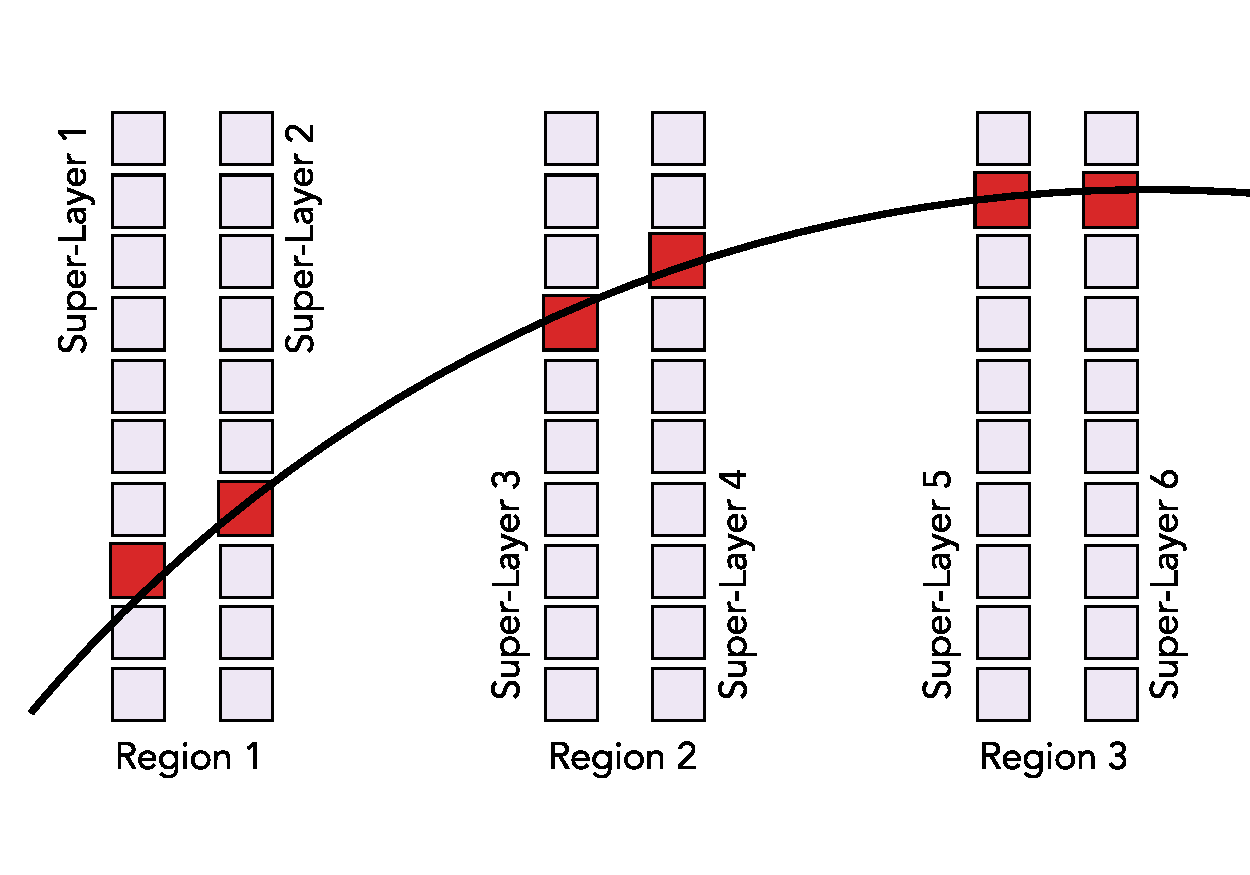
\includegraphics[width=2.1in]{images/dc_diagram.pdf}
 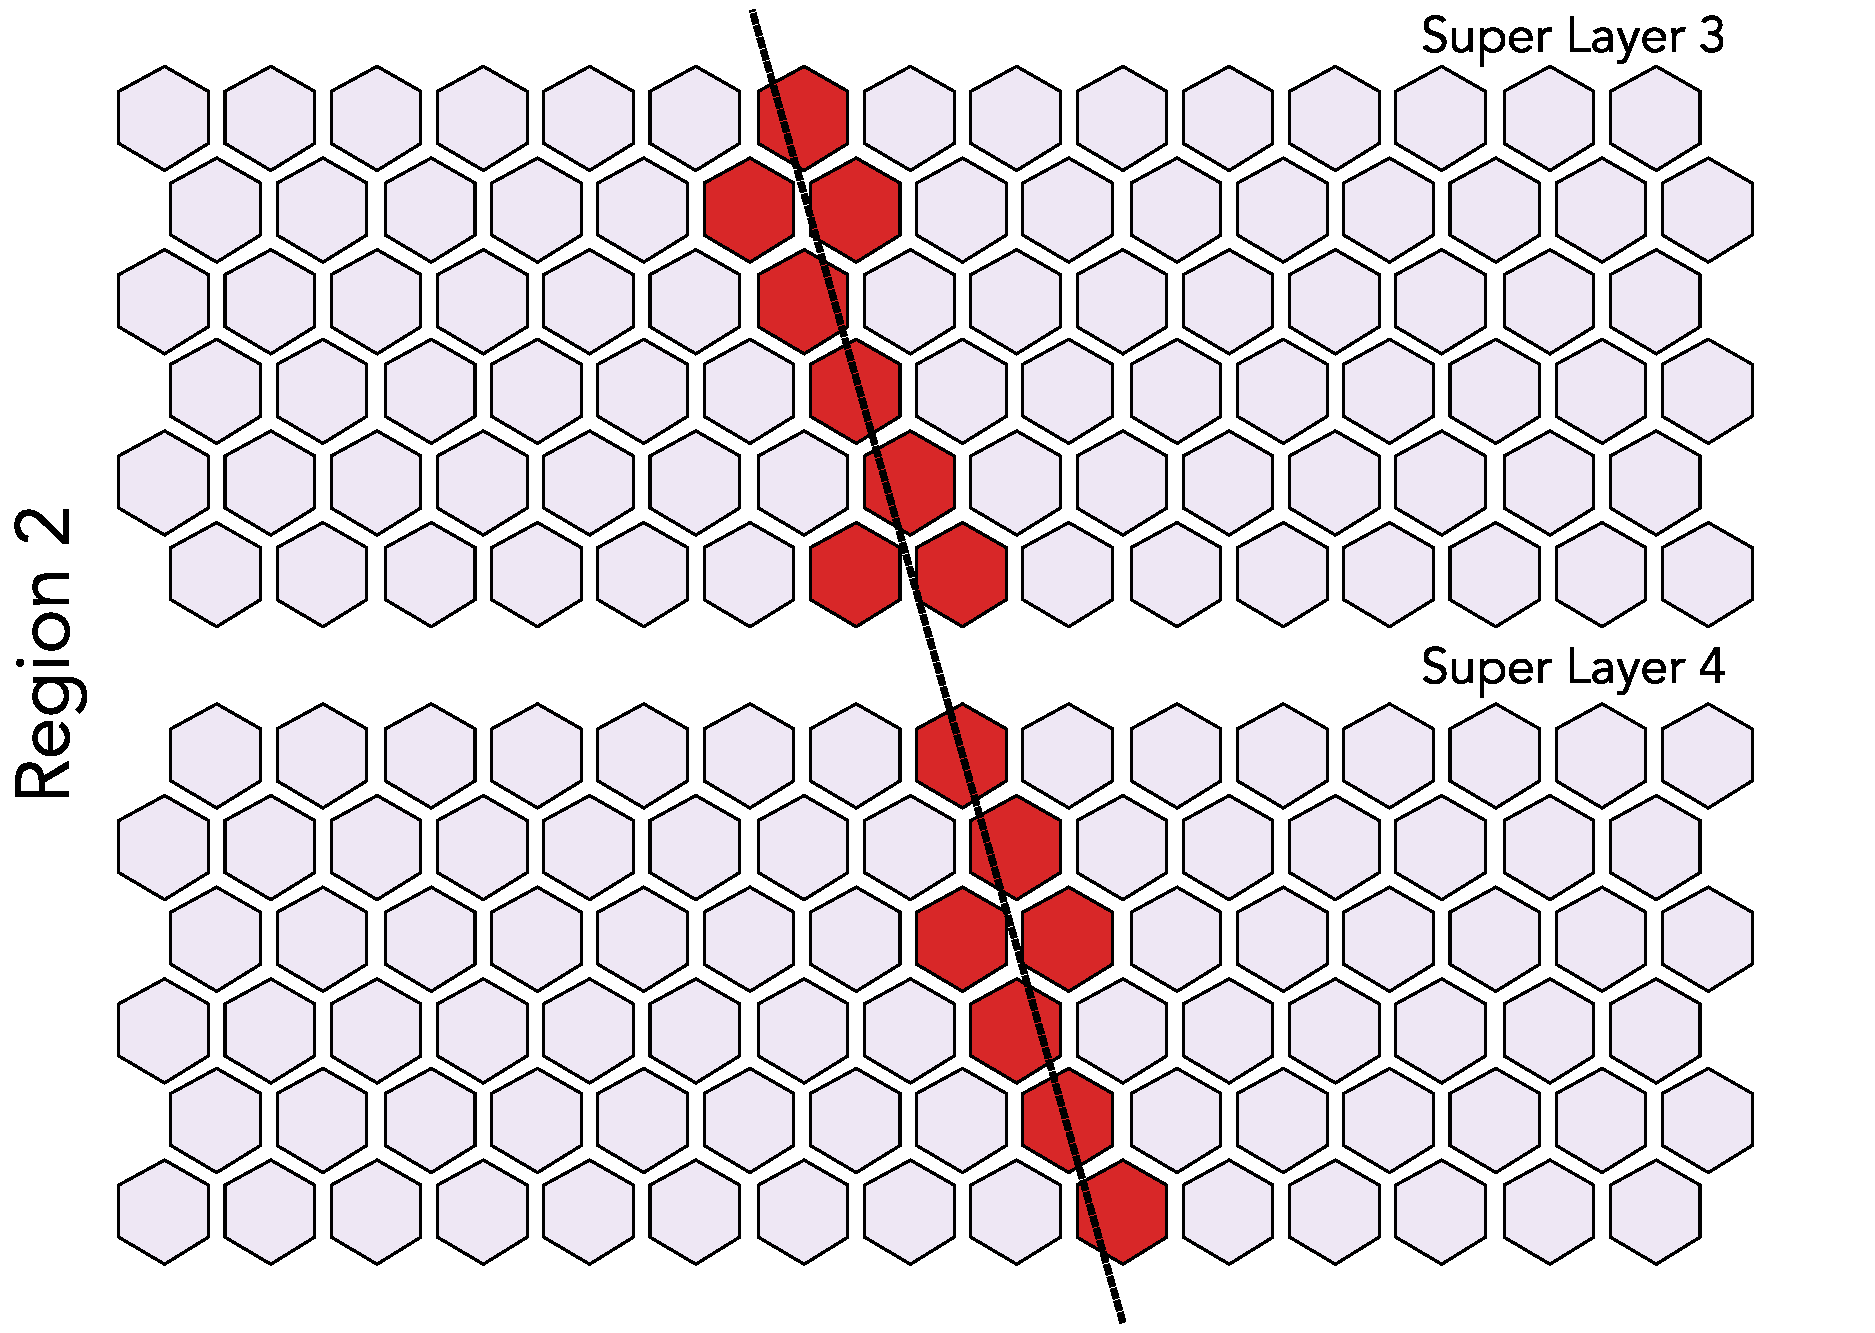
\includegraphics[width=2in]{images/region_2_diagram.pdf}
\caption {Schematic view of signals generated in the drift chambers when a particle passes through. 
The segments in each super-layer are shown along the trajectory of the track (left panel), and view 
of the activated cells in the two super-layers of one region along the track trajectory (right panel).}
 \label{dc:side_view}
 \end{center}
\end{figure}

Particles that originate at the interaction vertex travel through the magnetic field and pass through all 
three regions of the drift chambers in a given sector are reconstructed by tracking algorithms. First, 
in each super-layer adjacent wires with a signal are grouped together into clusters (called segments), 
shown in Figure~\ref{dc:side_view}. The positions of these clusters (segments) in each super-layer 
are used to fit the track trajectory to derive initial parameters, such as momentum and direction. 
After the initial selection, good track candidates are passed through Kalman filter~\cite{Kalman1960} 
 to further refine measured parameters.

\begin{figure}[!ht]
\begin{center}
 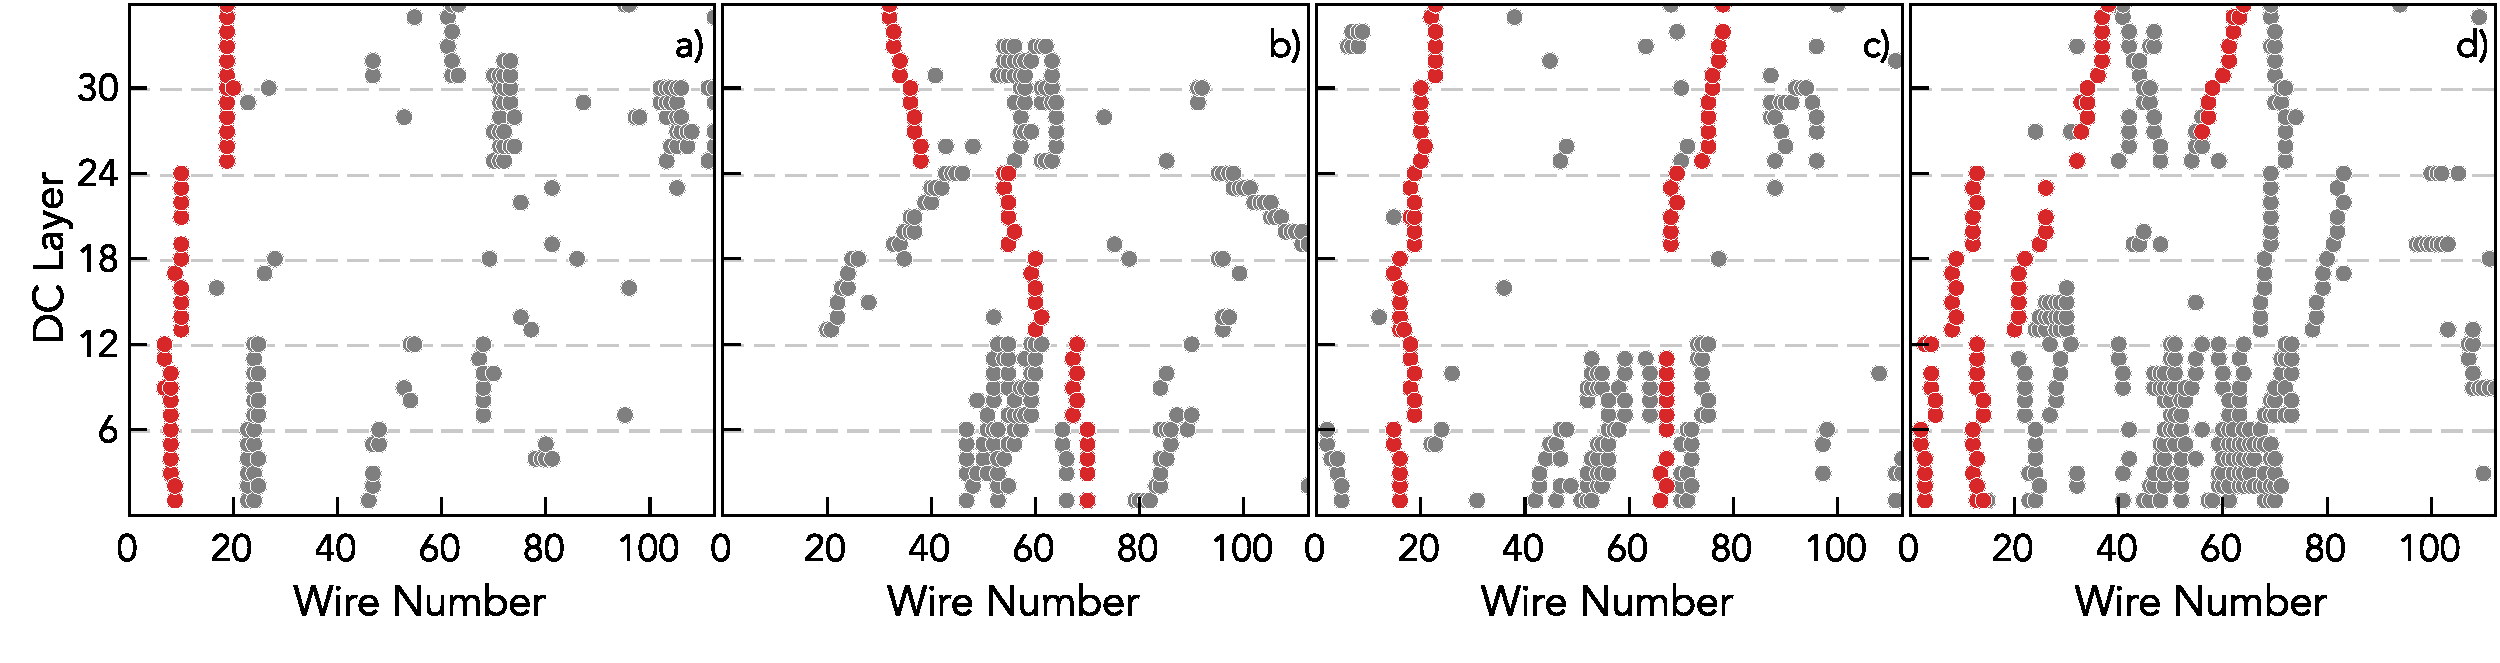
\includegraphics[width=4.2in]{images/figure_dc_examples.pdf}
\caption {Example of signals in drift chambers for four events. Each plot represents one sector with a 
36x112 matrix of wires. Background hits (in gray) are shown along with the hits of reconstructed 
identified tracks (in red). Dashed lines represent boundaries between super-layers.}
 \label{dc:events_sector}
 \end{center}
\end{figure}

For each beam-target interaction or ``event'', drift chambers produce many segments, some belonging 
to a track and some are background or partial trajectories of low-momentum tracks. In Figure~\ref{dc:events_sector} 
drift chamber signals in one sector are shown for four different  events, in each sector data are hits 
represented as a 36x112 matrix (36 layers and 112 wires per layer), showing all hits including those that 
were determined to be part of a track. 

Due to inefficiencies in the drift chambers, it is possible to have one missing segment along the trajectory 
of the particle, and the track has to be reconstructed using only 5 segments. An example of a 5-segment 
track is shown in Figure~\ref{dc:events_sector} c), where super-layer 3 does not have any segment detected. 
For these types of tracks, candidates have to be identified from a large number of combinatorics consisting 
of all combinations of clusters that form 5-segment candidates. 

%Tracking is computationally intensive and makes up $80\%-90\%$ of the total CLAS12 event processing 
%time (depending on background conditions and track multiplicity). The procedure of finding tracks from a 
%list of track candidates is where we found AI can provide real benefits. Such benefits include improved 
%accuracy in identifying good tracks and improved data processing speed by significantly reducing the 
%number of candidates that have to go through initial fitting and then through the Kalman filter. AI can also 
%help in identifying 5 super-layer track candidates.


 \subsection{Track Classifier}
 \label{track-classifier}
 
 %To determine what type of machine learning model works best with the CLAS12 drift chamber data, 
 %we investigated different types of models  \cite{Gavalian:2020oxg}, including Convolutional Neural 
 %Network (CNN), Extremely Randomized Trees (ERT), and 
 %Multi-Layer Perceptron (MLP). 
 
 A Multi-Layer Perceptron neural network is used for the CLAS12 track identification  \cite{Gavalian:2020oxg}. 
 The implemented architecture is shown in Figure~\ref{mlp:architecture}, where an input layer with 6 
 nodes are used (each node representing the average wire position of the segment in the super-layer) and 3 
 output nodes for the classes ``positive track'', ``negative track'' and ``false track''.
 
 \begin{figure}[!ht]
\begin{center}
  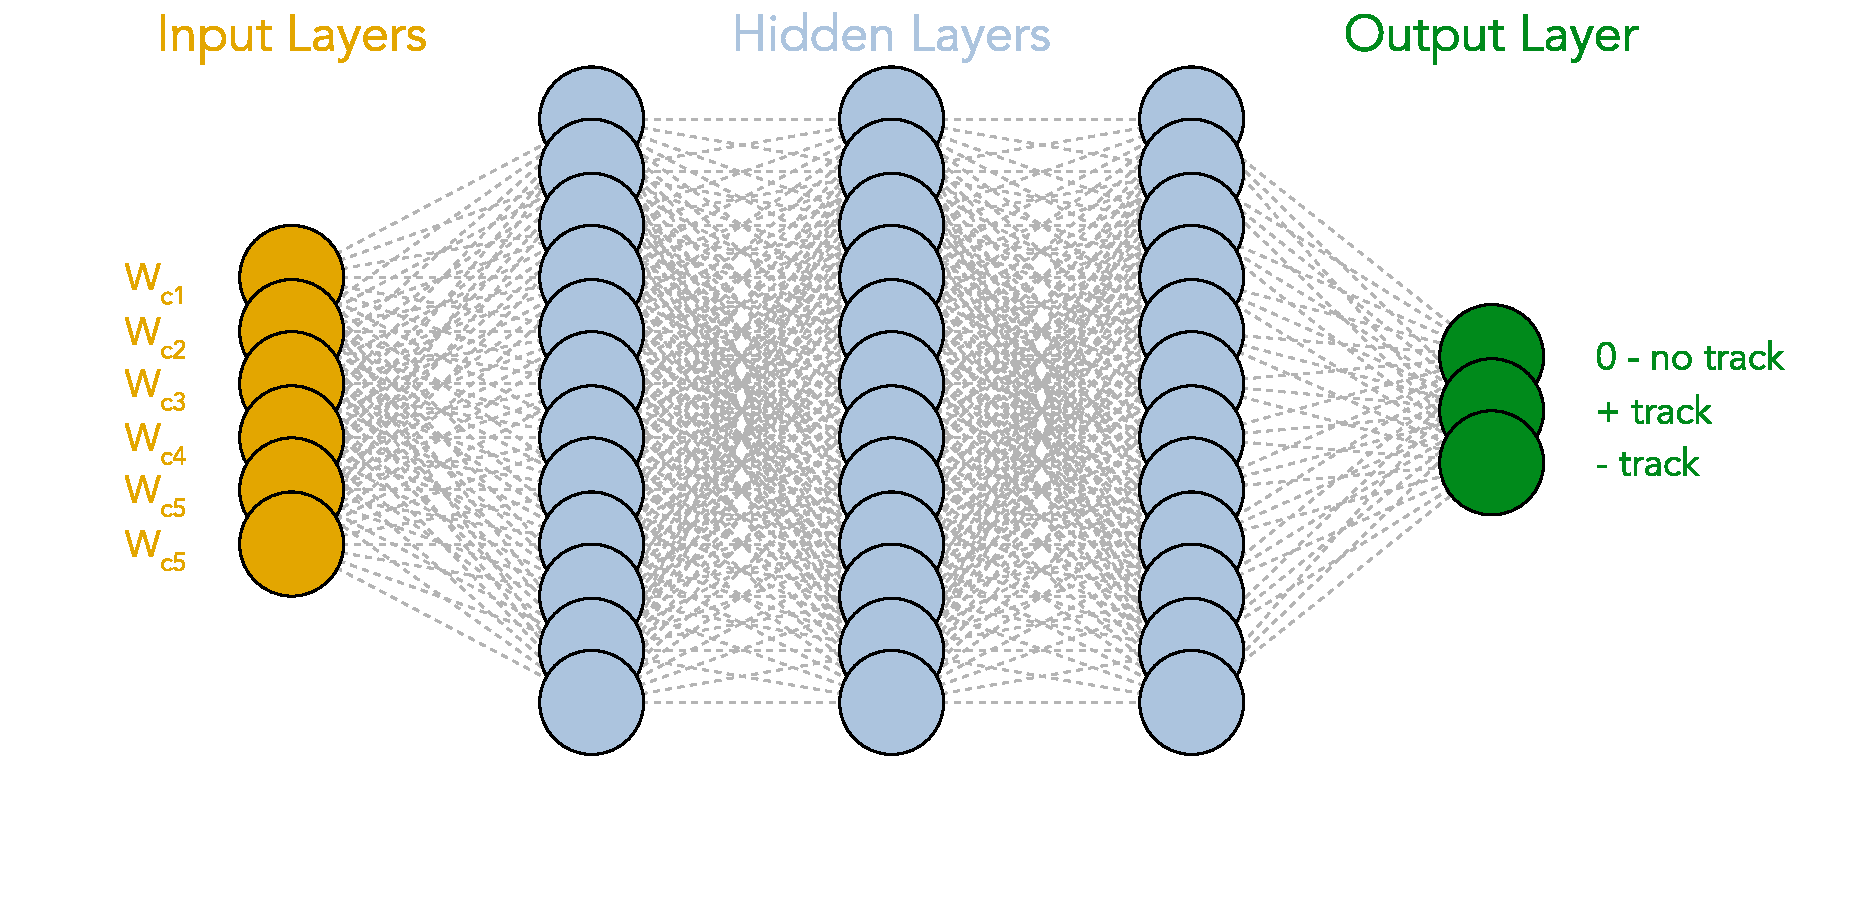
\includegraphics[width=2.1in]{images/mlp_diagram.pdf}
  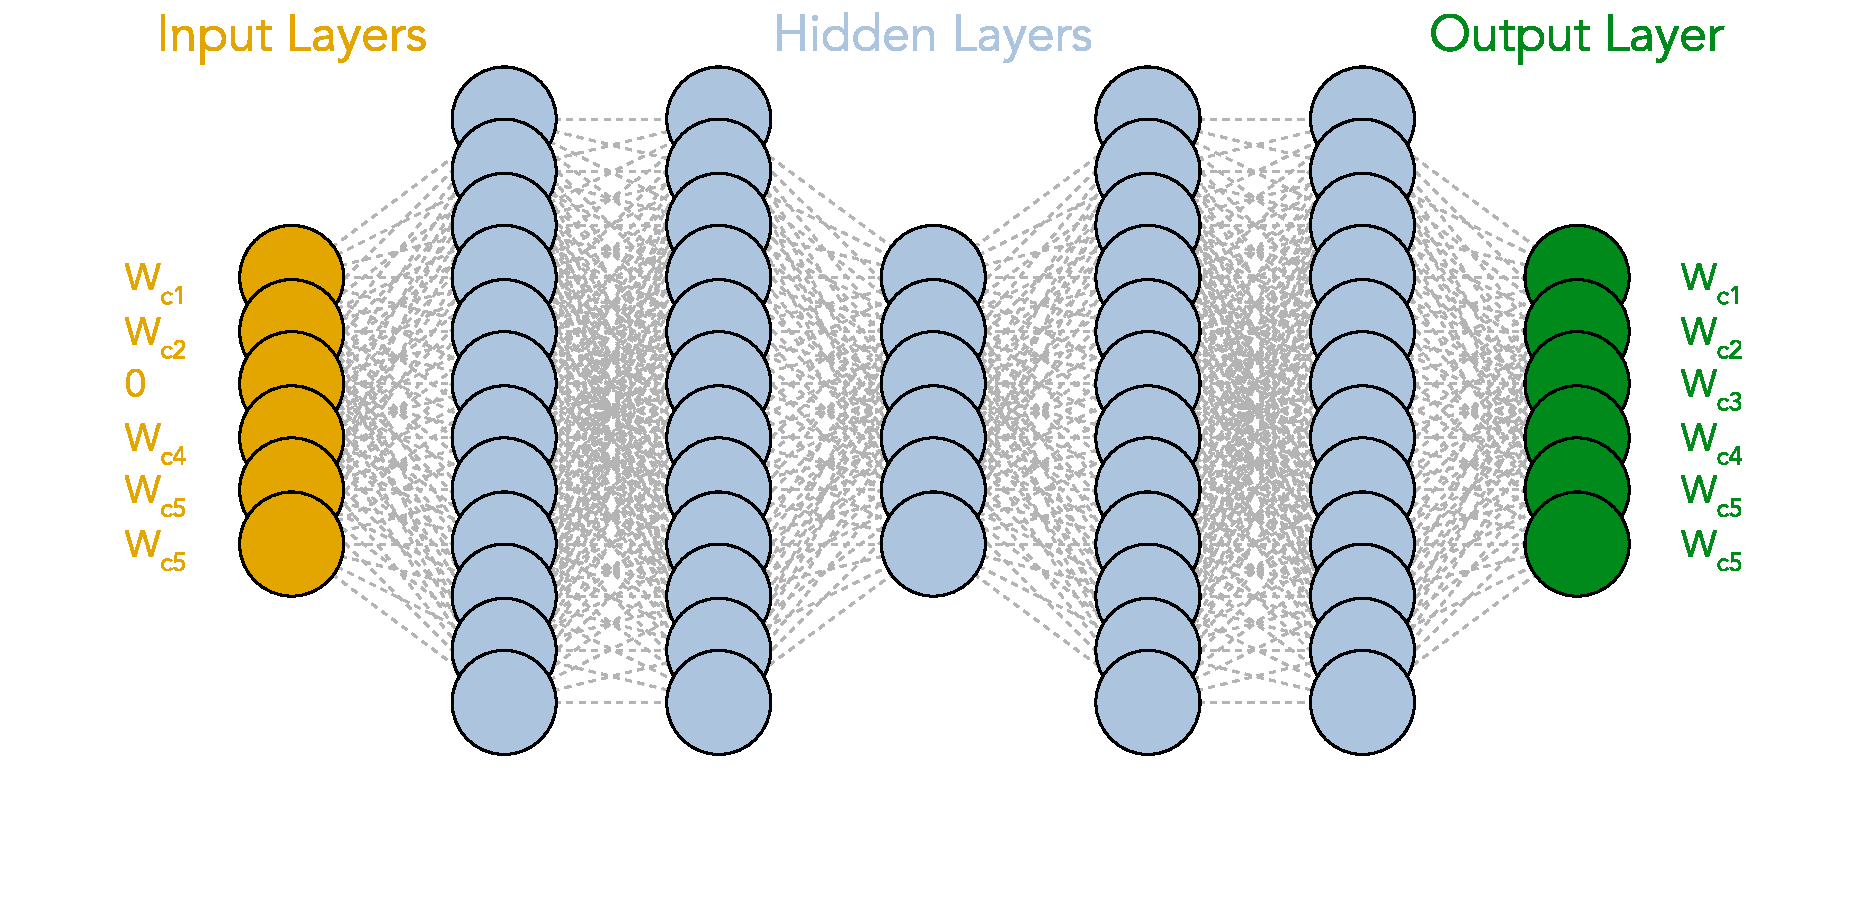
\includegraphics[width=2.1in]{images/aue_diagram.pdf}
\caption {a) Architecture of Multi-Layer Perceptron used for track classification. The network has 6 input nodes,
corresponding to the average wire positions of the segment in each super-layer, three hidden layers with 12 nodes 
in each, and 3 output nodes. b) Corruption-recovery auto-encoder architecture with 6 input nodes representing track segments 
mean wire values with one of the values is set to 0, and 6 output nodes with the correct value for the node 
that has 0 in the input. }
 \label{mlp:architecture}
 \end{center}
\end{figure}

The network is trained using a sample of tracks reconstructed by the conventional algorithm, selected with 
$\chi^2$ cuts to retain the highest quality ones, which are fed to the network with their respective labels 
(i.e. positive or negative tracks). For false tracks, a combination of segments (6 segments forming a track 
candidate) that was not identified as a track by the conventional algorithm is chosen.
 
 \subsection{Corruption Auto-Encoder}
 
 \begin{figure}[!ht]
\begin{center}
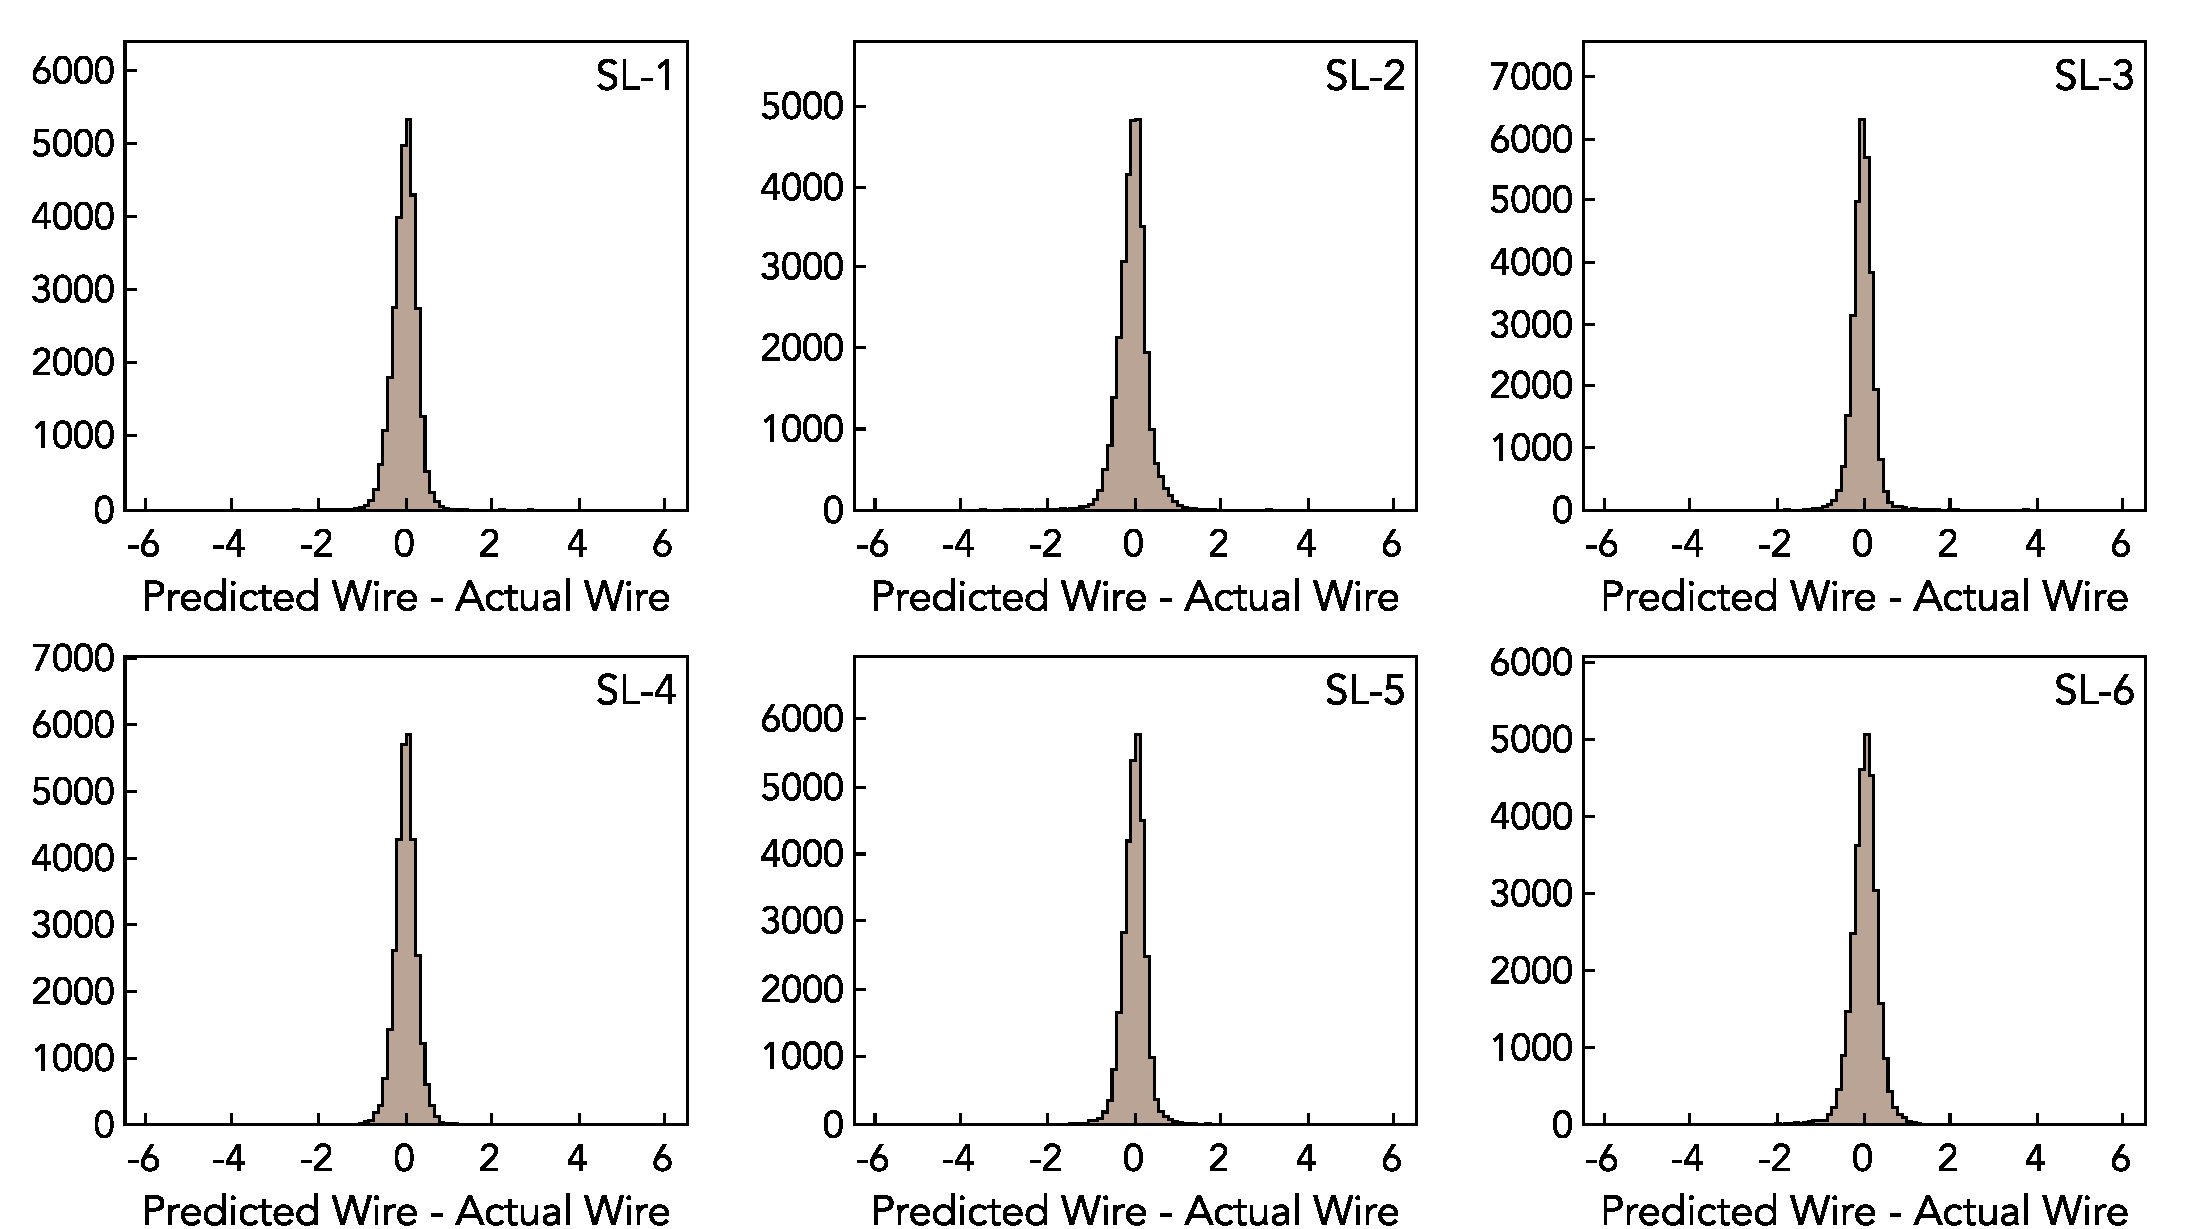
\includegraphics[width=4.0in]{images/encoder_performance.pdf}
\caption {Performance of corruption recovery auto-encoder for each of six super-layers. The difference between predicted and actual 
wire position is shown for all super-layers. The average accuracy of wire position prediction is  $0.36$ wire.}
 \label{autoencoder:performance}
 \end{center}
\end{figure}

A second neural network was developed to fix the corruption in possible track candidates due to 
inefficiencies of drift chambers. This network was used to identify track candidates which have one of 
the segments missing. We used an auto-encoder architecture to implement the corruption-recovery 
neural network \cite{Gavalian:2020xmc}. The structure of the network can be seen in 
Figure~\ref{mlp:architecture}, with 6 input nodes and 6 output nodes.

To train the corruption auto-encoder network the same sample used for the classifier training was used.
The output for the network was set to the good track parameters (where all 6 segments have non-zero values) 
and the input was modified by setting one of the nodes (randomly) to zero. The network learns to fix the node 
containing zero, by assigning it a value based on the other 5 segment values. 

The test results of the trained network are shown in Figure~\ref{autoencoder:performance}, where the 
difference between the true value of the segment position and the one reconstructed by the network is 
plotted, showing a reconstruction accuracy of $0.36$ wires. In Figure~\ref{autoencoder:performance} 
this difference is shown for each super-layer that was corrupted in the input. As can be seen, 
the performance of the network is uniform across all super-layers.

\subsection{Track Identification Workflow}
\label{track-identification-workflow}

 Track identification consists of two phases, programmed to be done in two passes. In the first pass 
 over the data, signals from each sector of drift chambers are analyzed to create a track candidate list, 
 each consisting of 6 segments. The resulting track candidates are evaluated by the classifier neural 
 network and are assigned a probability of being either a positive or negative track. 
 
 %The list of track 
 %candidates is sorted by probability and passed to another algorithm that is responsible for removing 
 %tracks that have a lower probability of being a "good" track and have clusters that are shared with a 
 %higher-probability candidate. 

%In this procedure, the algorithm iterates over-track candidates sorted according to the probability of 
%being a good track. Iteration starts at position number 2 and runs to the end of the list. Candidates that 
%share a cluster with candidates at position number 1 are removed from the list. Track candidate at position 
%1 is moved from the track candidate list into the identified track list. This procedure is repeated until 
%there are no track candidates left in the candidate list.

 \begin{figure}[!h]
\begin{center}
 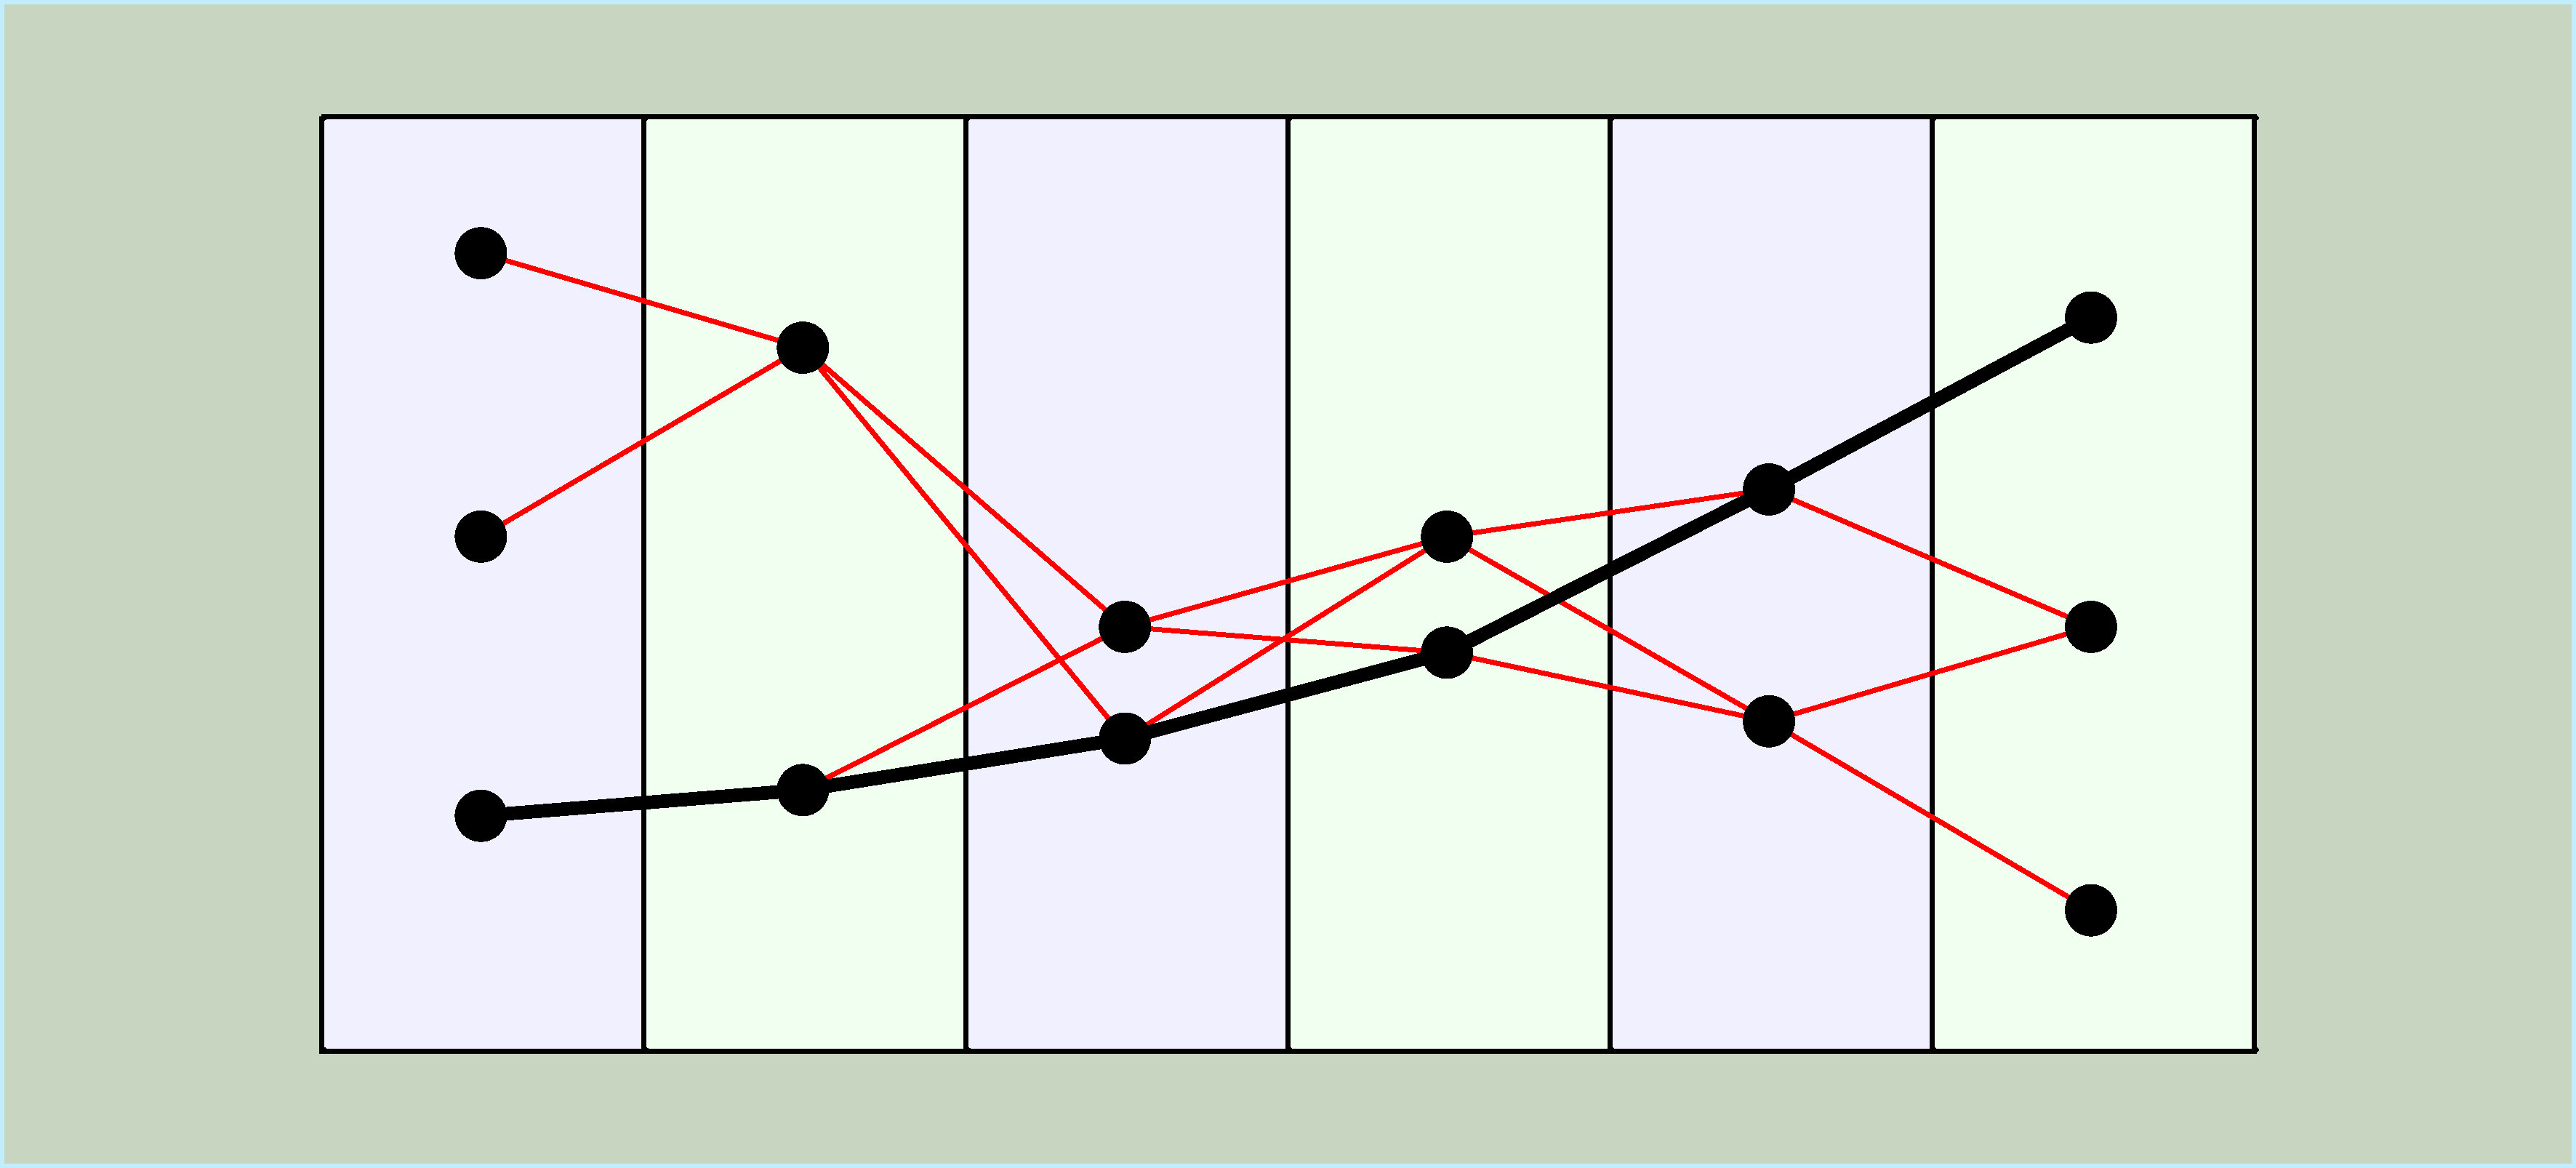
\includegraphics[angle=90,width=0.8in]{images/iden_6_sl.pdf}
  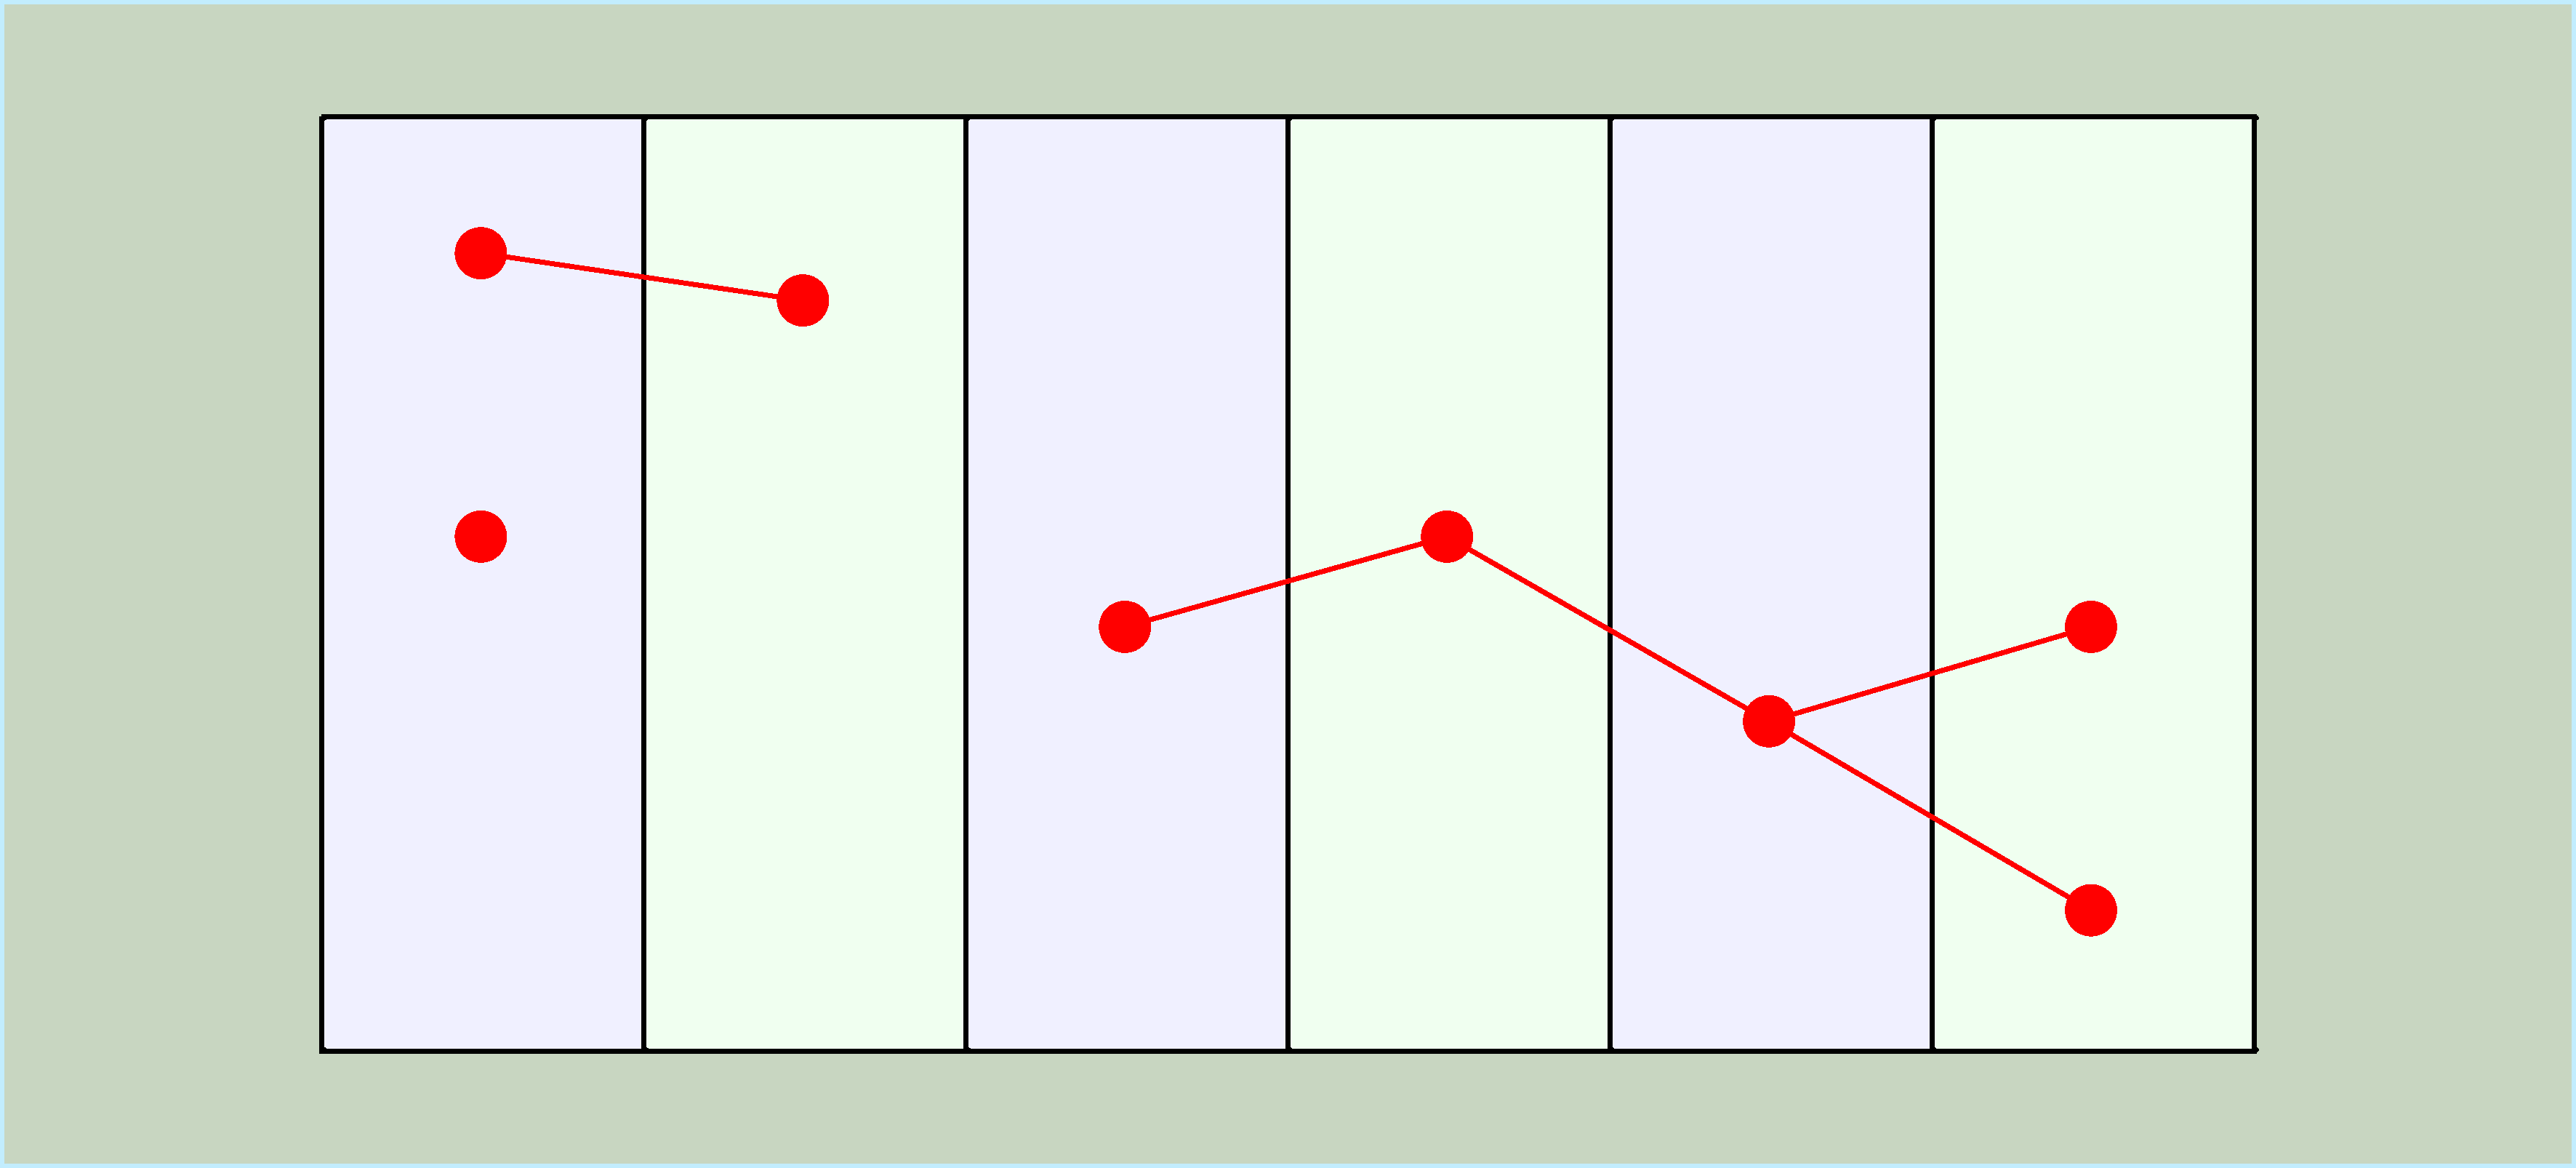
\includegraphics[angle=90,width=0.8in]{images/iden_5_sl_a.pdf}
    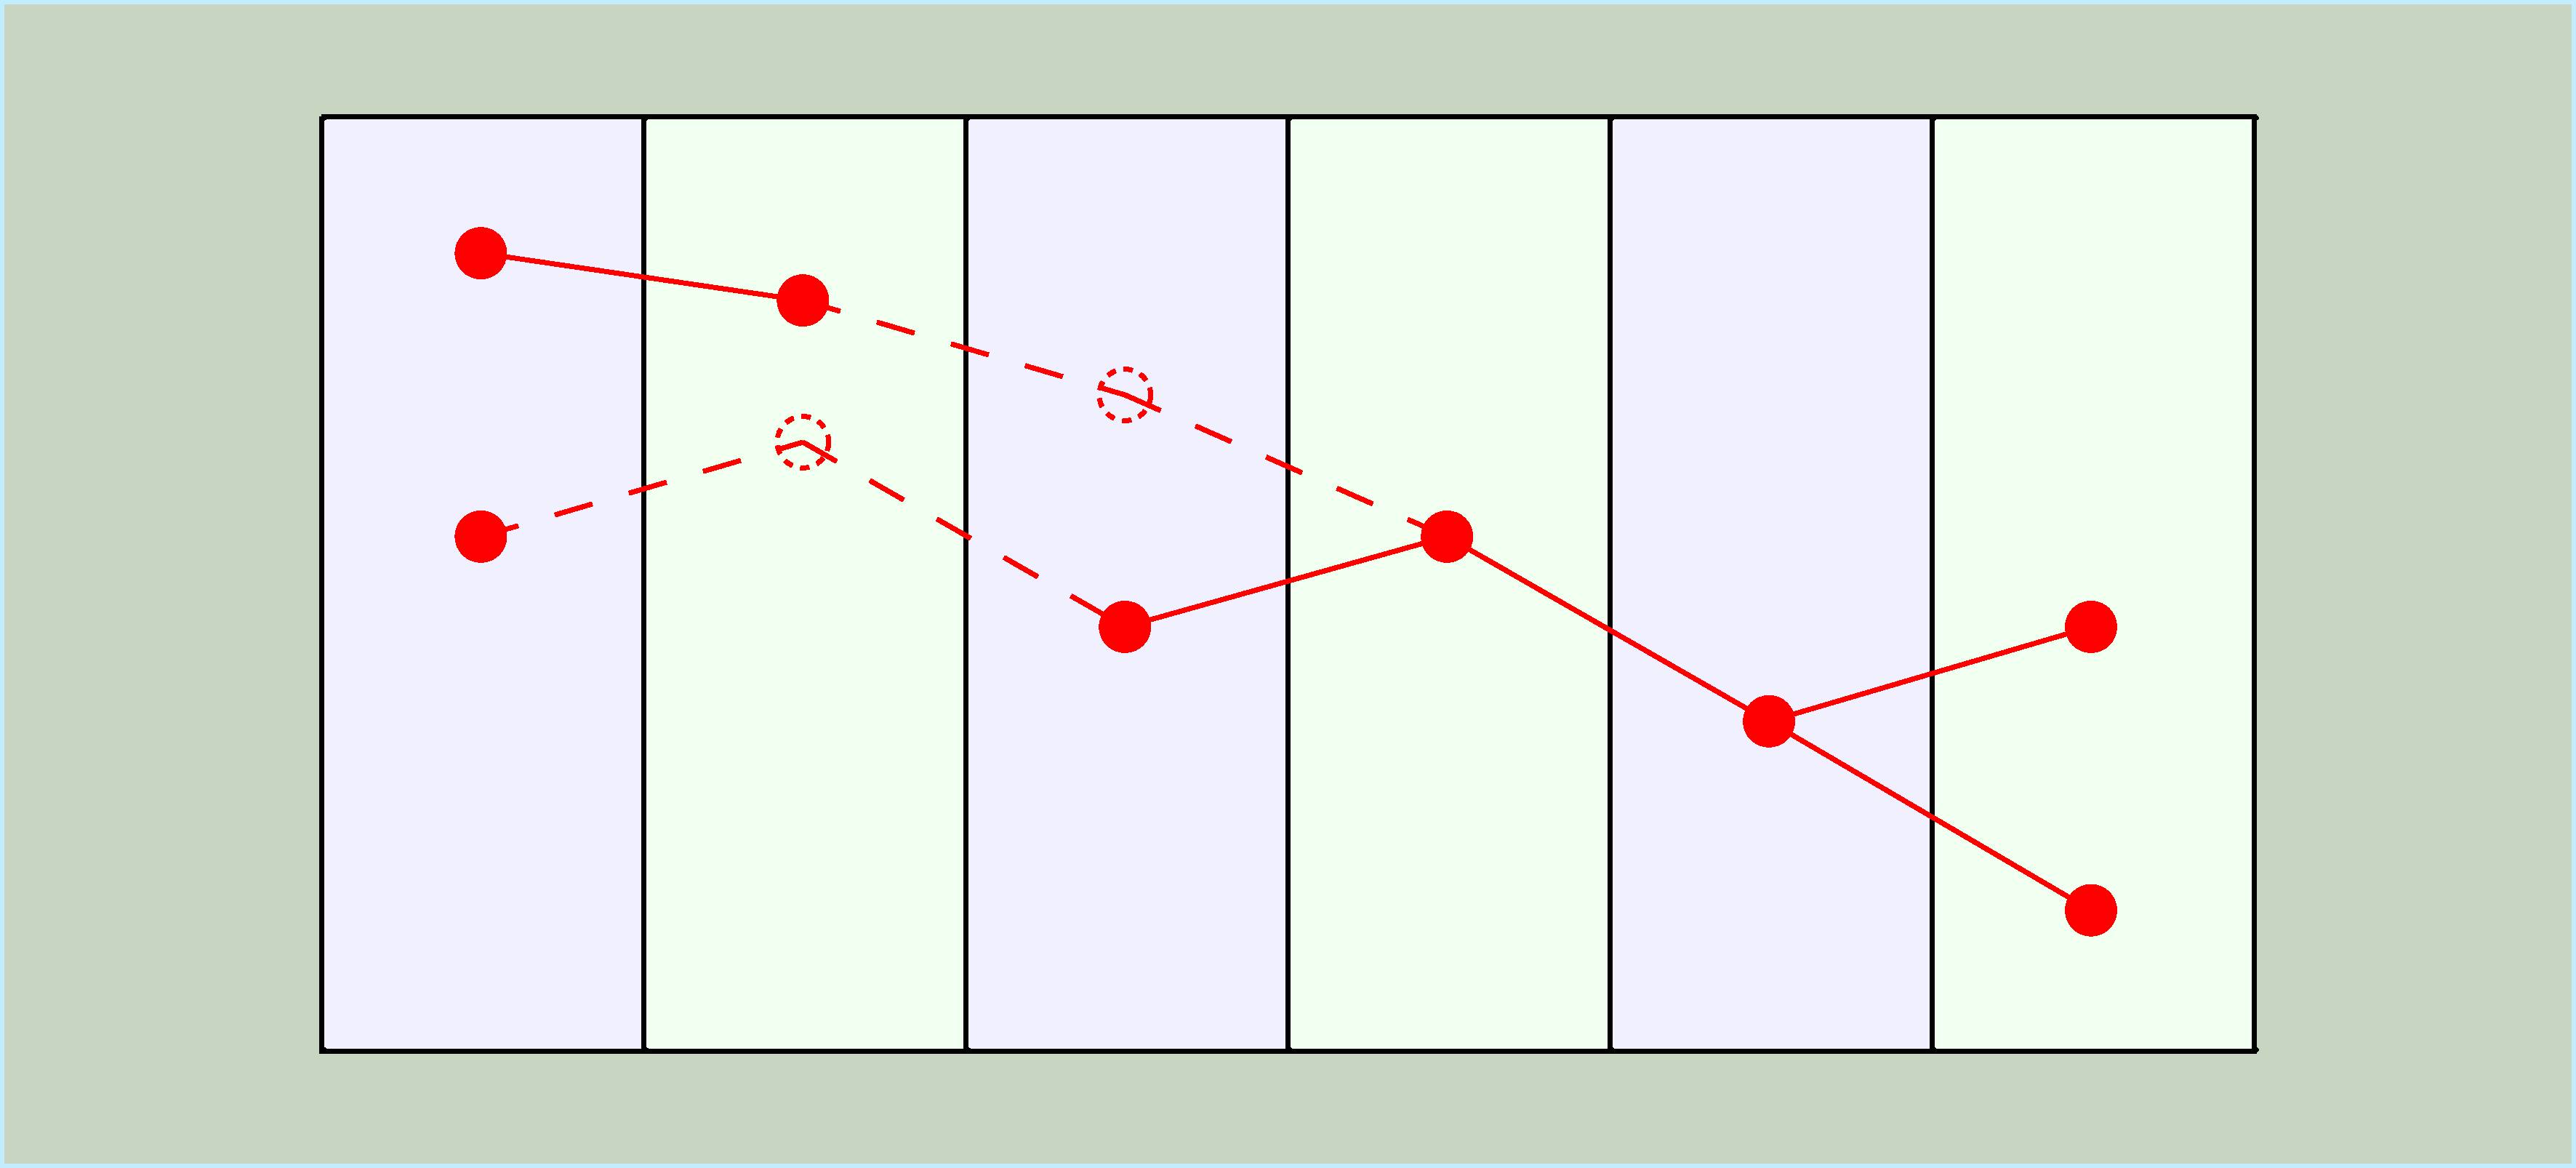
\includegraphics[angle=90,width=0.8in]{images/iden_5_sl_b.pdf}
      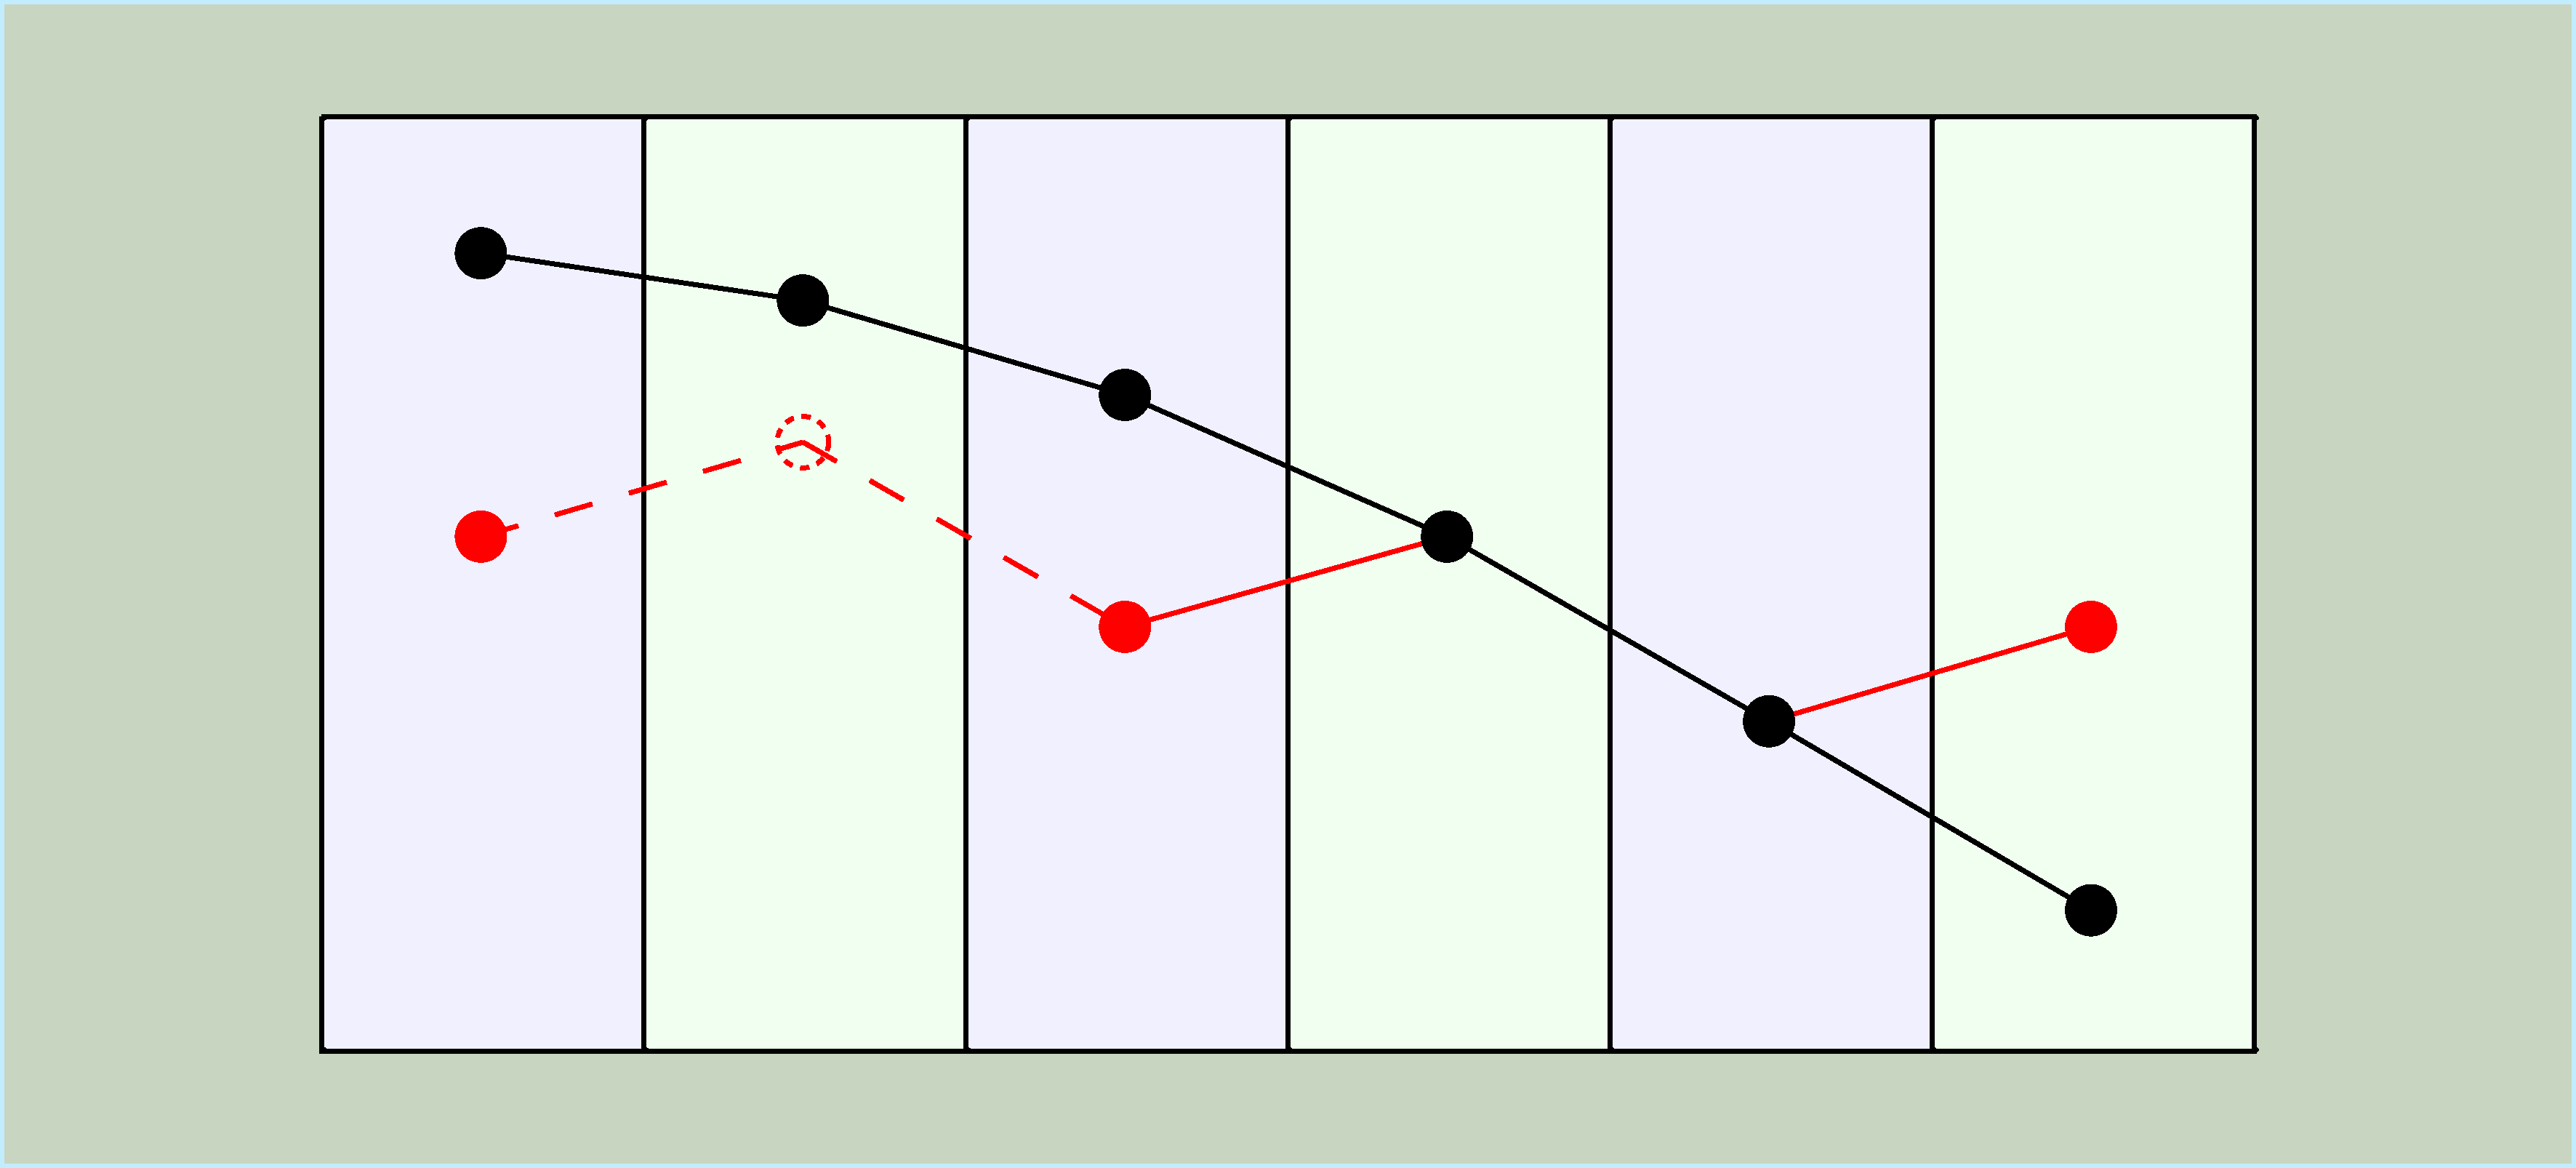
\includegraphics[angle=90,width=0.8in]{images/iden_5_sl_c.pdf}
            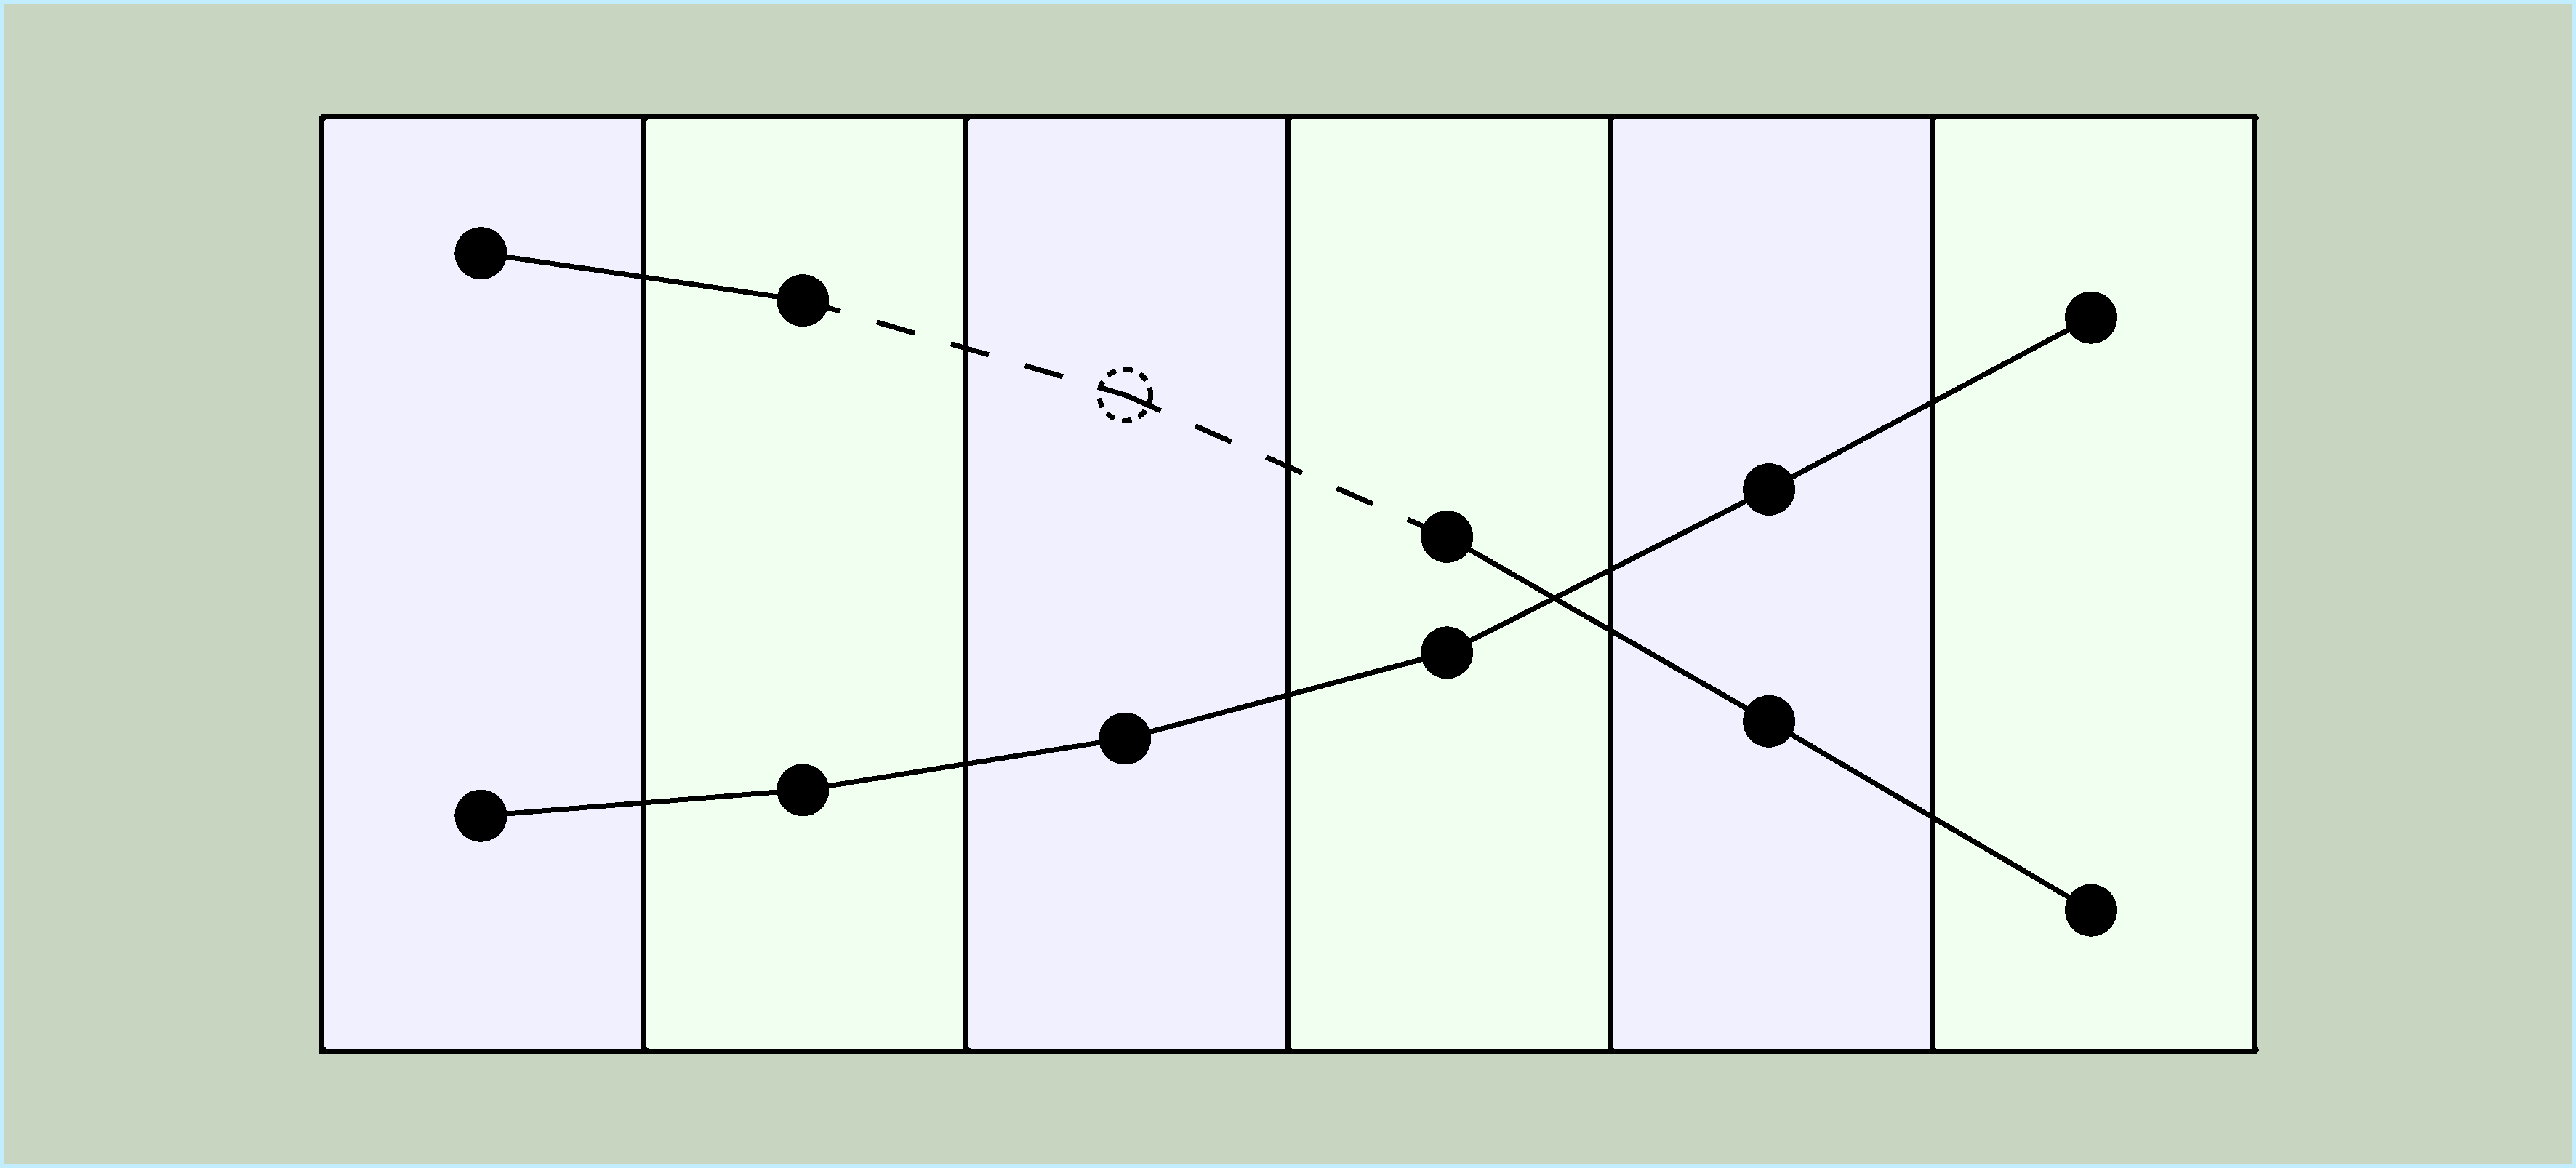
\includegraphics[angle=90,width=0.8in]{images/iden_5_sl_d.pdf}
            
\caption {Stages of Neural Network track identification procedure. 1) identifying 6 super-layer tracks. 2) 
removing all hits belonging to an identified track and constructing 5 super-layer track candidates. 
3) generating pseudo-clusters for 5 super-layer track candidates using corruption fixing auto-encoder. 
4) identify good track candidates from the list of 6 super-layer (one of the super-layers is a pseudo-cluster) 
track candidates. 5) isolate both identified (6 super-layer and 5 super-layer) tracks  for further fitting with 
Kalman-Filter.}
 \label{network:procedure}
 \end{center}
\end{figure}

The second stage of track identification starts by constructing a list of track candidates with combinations 
of 5 clusters out of 6 from all existing clusters (one per super-layer). The candidates that share a cluster with 
tracks identified at the first stage of classification are removed from the list. For each track candidate with a 
missing cluster in one of the super-layers, a pseudo-cluster is generated using the Corruption Auto-Encoder 
Network and the missing super-layer cluster are assigned the inferred value, hence turning all track candidates 
into 6 cluster track candidates. The cured (or fixed) track candidate list is finally passed to the track classifier 
module described above, which evaluates the list by isolating candidates with the highest probability of being a 
good track. 

\subsection{Physics Impact}
\label{physics-impact}

 \begin{figure}[!ht]
\begin{center}
 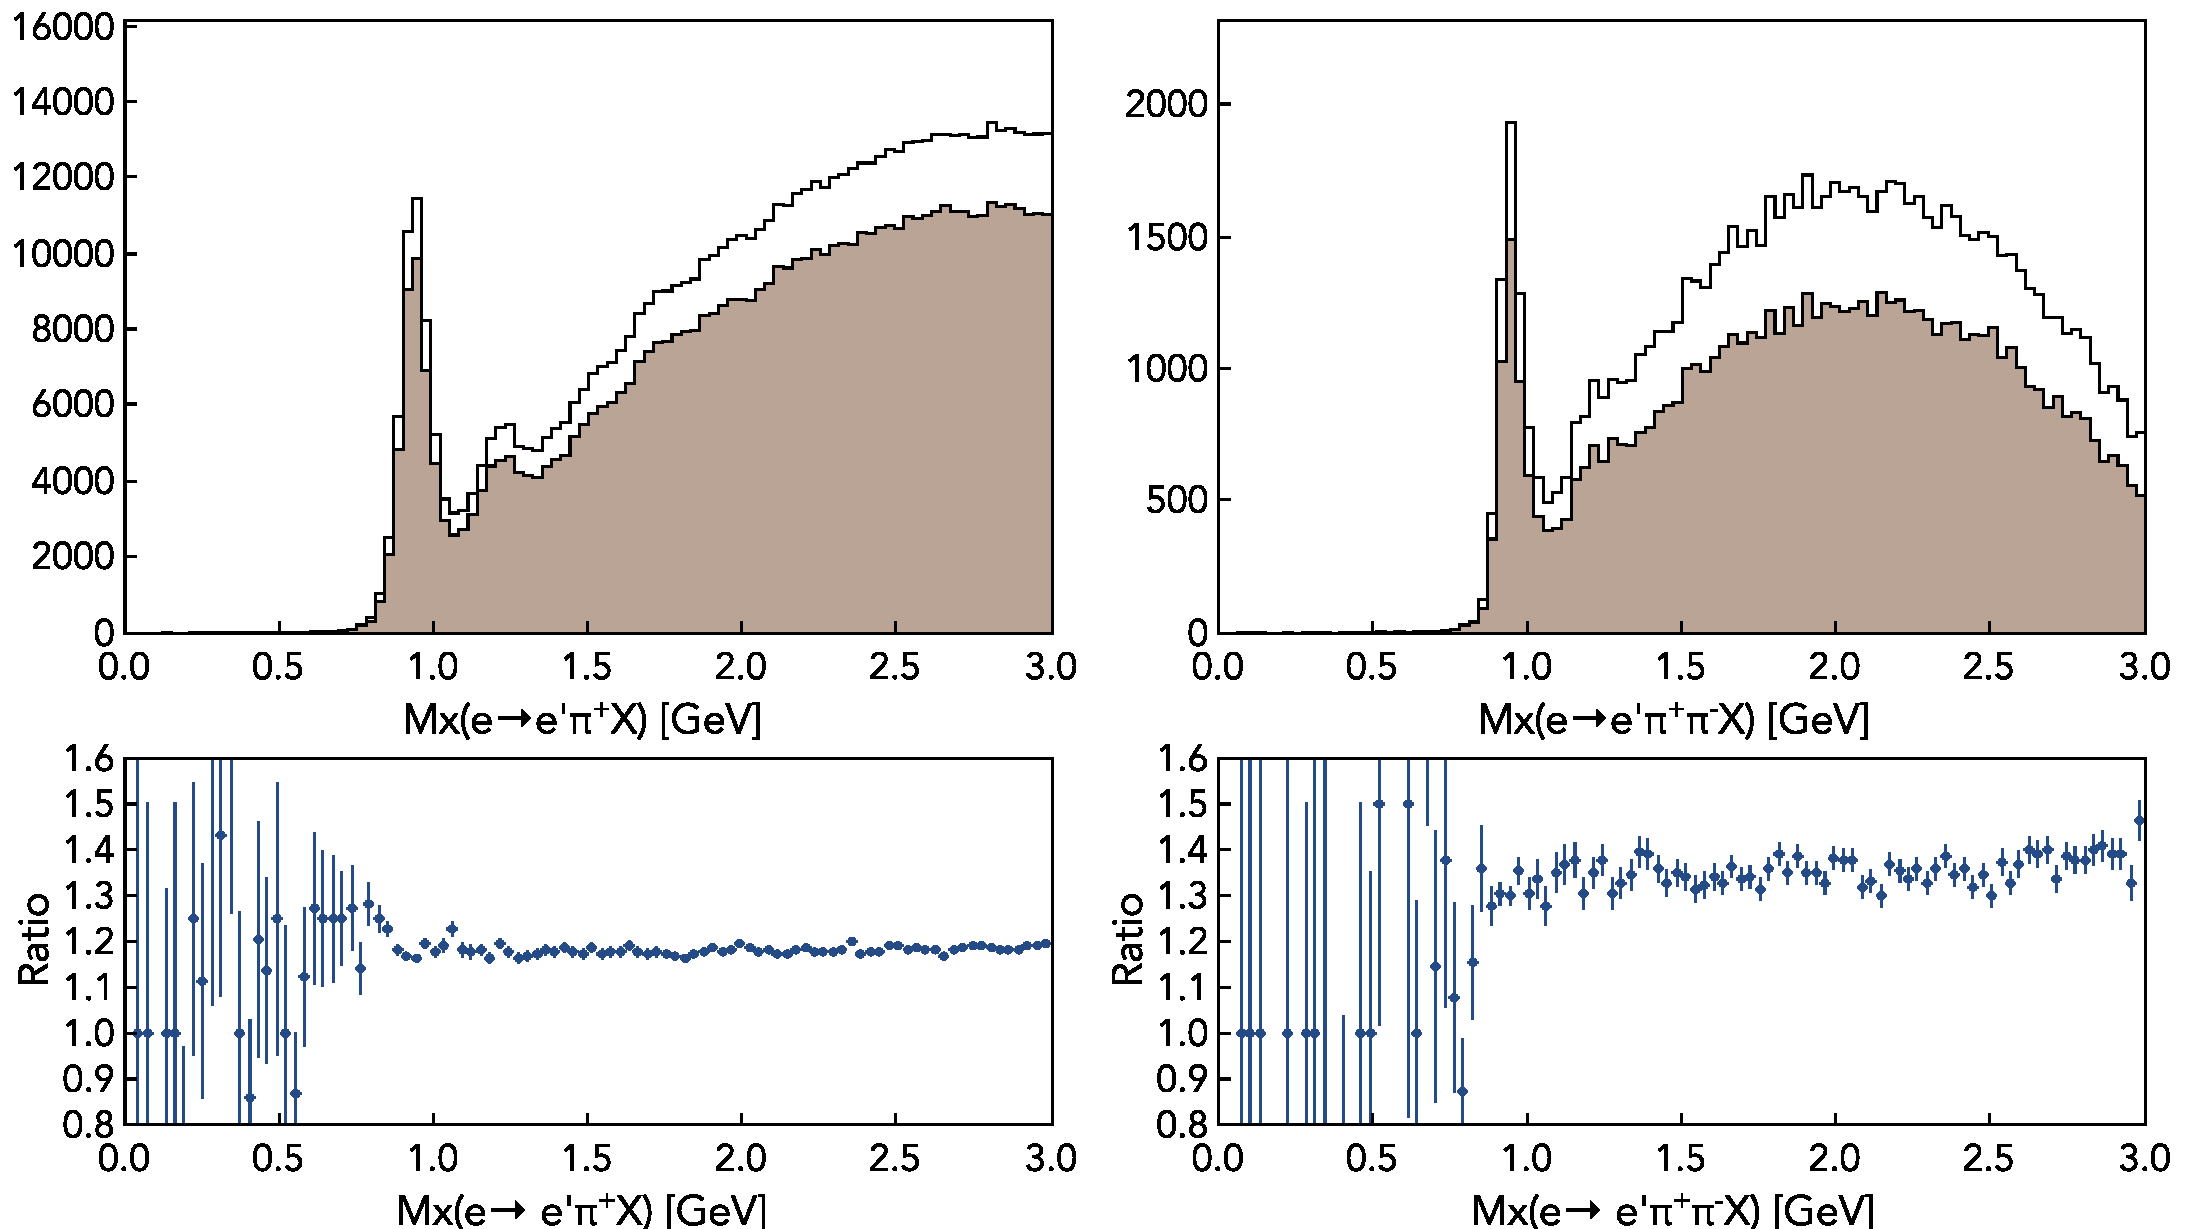
\includegraphics[width=4.in]{images/physics_scan.pdf}
\caption {Reconstructed missing mass distribution for $H(e,e'\pi^+X)$ and $H(e,e'\pi^+\pi^-X)$ 
reactions (top row) using the conventional track reconstruction algorithm (filled histogram) and  
AI-assisted track reconstruction (black line histogram). The ratios of the two histograms are shown 
on the bottom row. }
 \label{physics:outcome}
 \end{center}
\end{figure}

To measure the implications of track reconstruction efficiency improvements on physics analysis, 
we considered two event topologies with two and three particles in the final state, respectively. 
The data for analysis were taken with $10.6~GeV$ electron beam incident on $5~cm$ liquid 
hydrogen target, with a beam current of $45~nA$. 
We selected events where an electron was detected in the forward detector, and then isolated 
events where there was an additional positively charged pion ($\pi^+$) along with an electron 
and no other charged particle. The second topology required two pions along with the electron, 
one positively charged and one negatively charged. The two chosen topologies are denoted by 
$H(e,e'\pi^+X)$ and $H(e,e'\pi^+\pi^-X)$. In both cases, there is a visible peak of a missing nucleon
in the missing mass distribution of the detected final state, which we can use to measure the impact 
of efficiency on physics outcome. 

The distributions of missing mass for both final state topologies are shown in Figure~\ref{physics:outcome}, where the plots 
on the top row are missing mass of $H(e,e'\pi^-X)$ and $H(e,e'\pi^+\pi^-X)$, where the filled histogram is calculated from 
particles reconstructed by the conventional tracking algorithm, and the histogram with a black outline is the same distributions 
calculated from particles that were reconstructed using a suggestion from Artificial Intelligence. As can be seen from the figure, 
there is a significant increase in the number of events in the region of the nucleon peak for AI-assisted
tracking. The ratios of the two histograms (AI-assisted divided by conventional)
Figure~\ref{physics:outcome} shows the increase in statistics is uniform over the whole range of the 
missing mass indicating no systematic abnormalities for AI-assisted tracking. The ratio also indicates that there is an increase 
in the number of events of about $15\%$ for $H(e,e'\pi^+X)$ final state and $30-35\%$ for the $H(e,e'\pi^+\pi^-X)$
final state. 
%Further studies show that improvements in statistics are larger for higher luminosity (higher incident beam current), 
%which is consistent with our studies of increased efficiency of single-particle reconstruction.

\section{Drift Chamber De-noising using Convolutional Auto-Encoders}
\label{dc-denoising}

The charged particle tracking relies on isolating clusters in each DC super-layer to identify tracks from the combination of clusters.
Accidental hits in drift chambers can, which increase with the luminosity, can lead to decreased efficiency of cluster identification, which 
in turn, leads to a decrease in track finding efficiency. A new approach with neural networks is used to clean raw data from drift chambers 
prior to applying the clustering algorithm. 

\begin{figure}[!h]
\begin{center}
 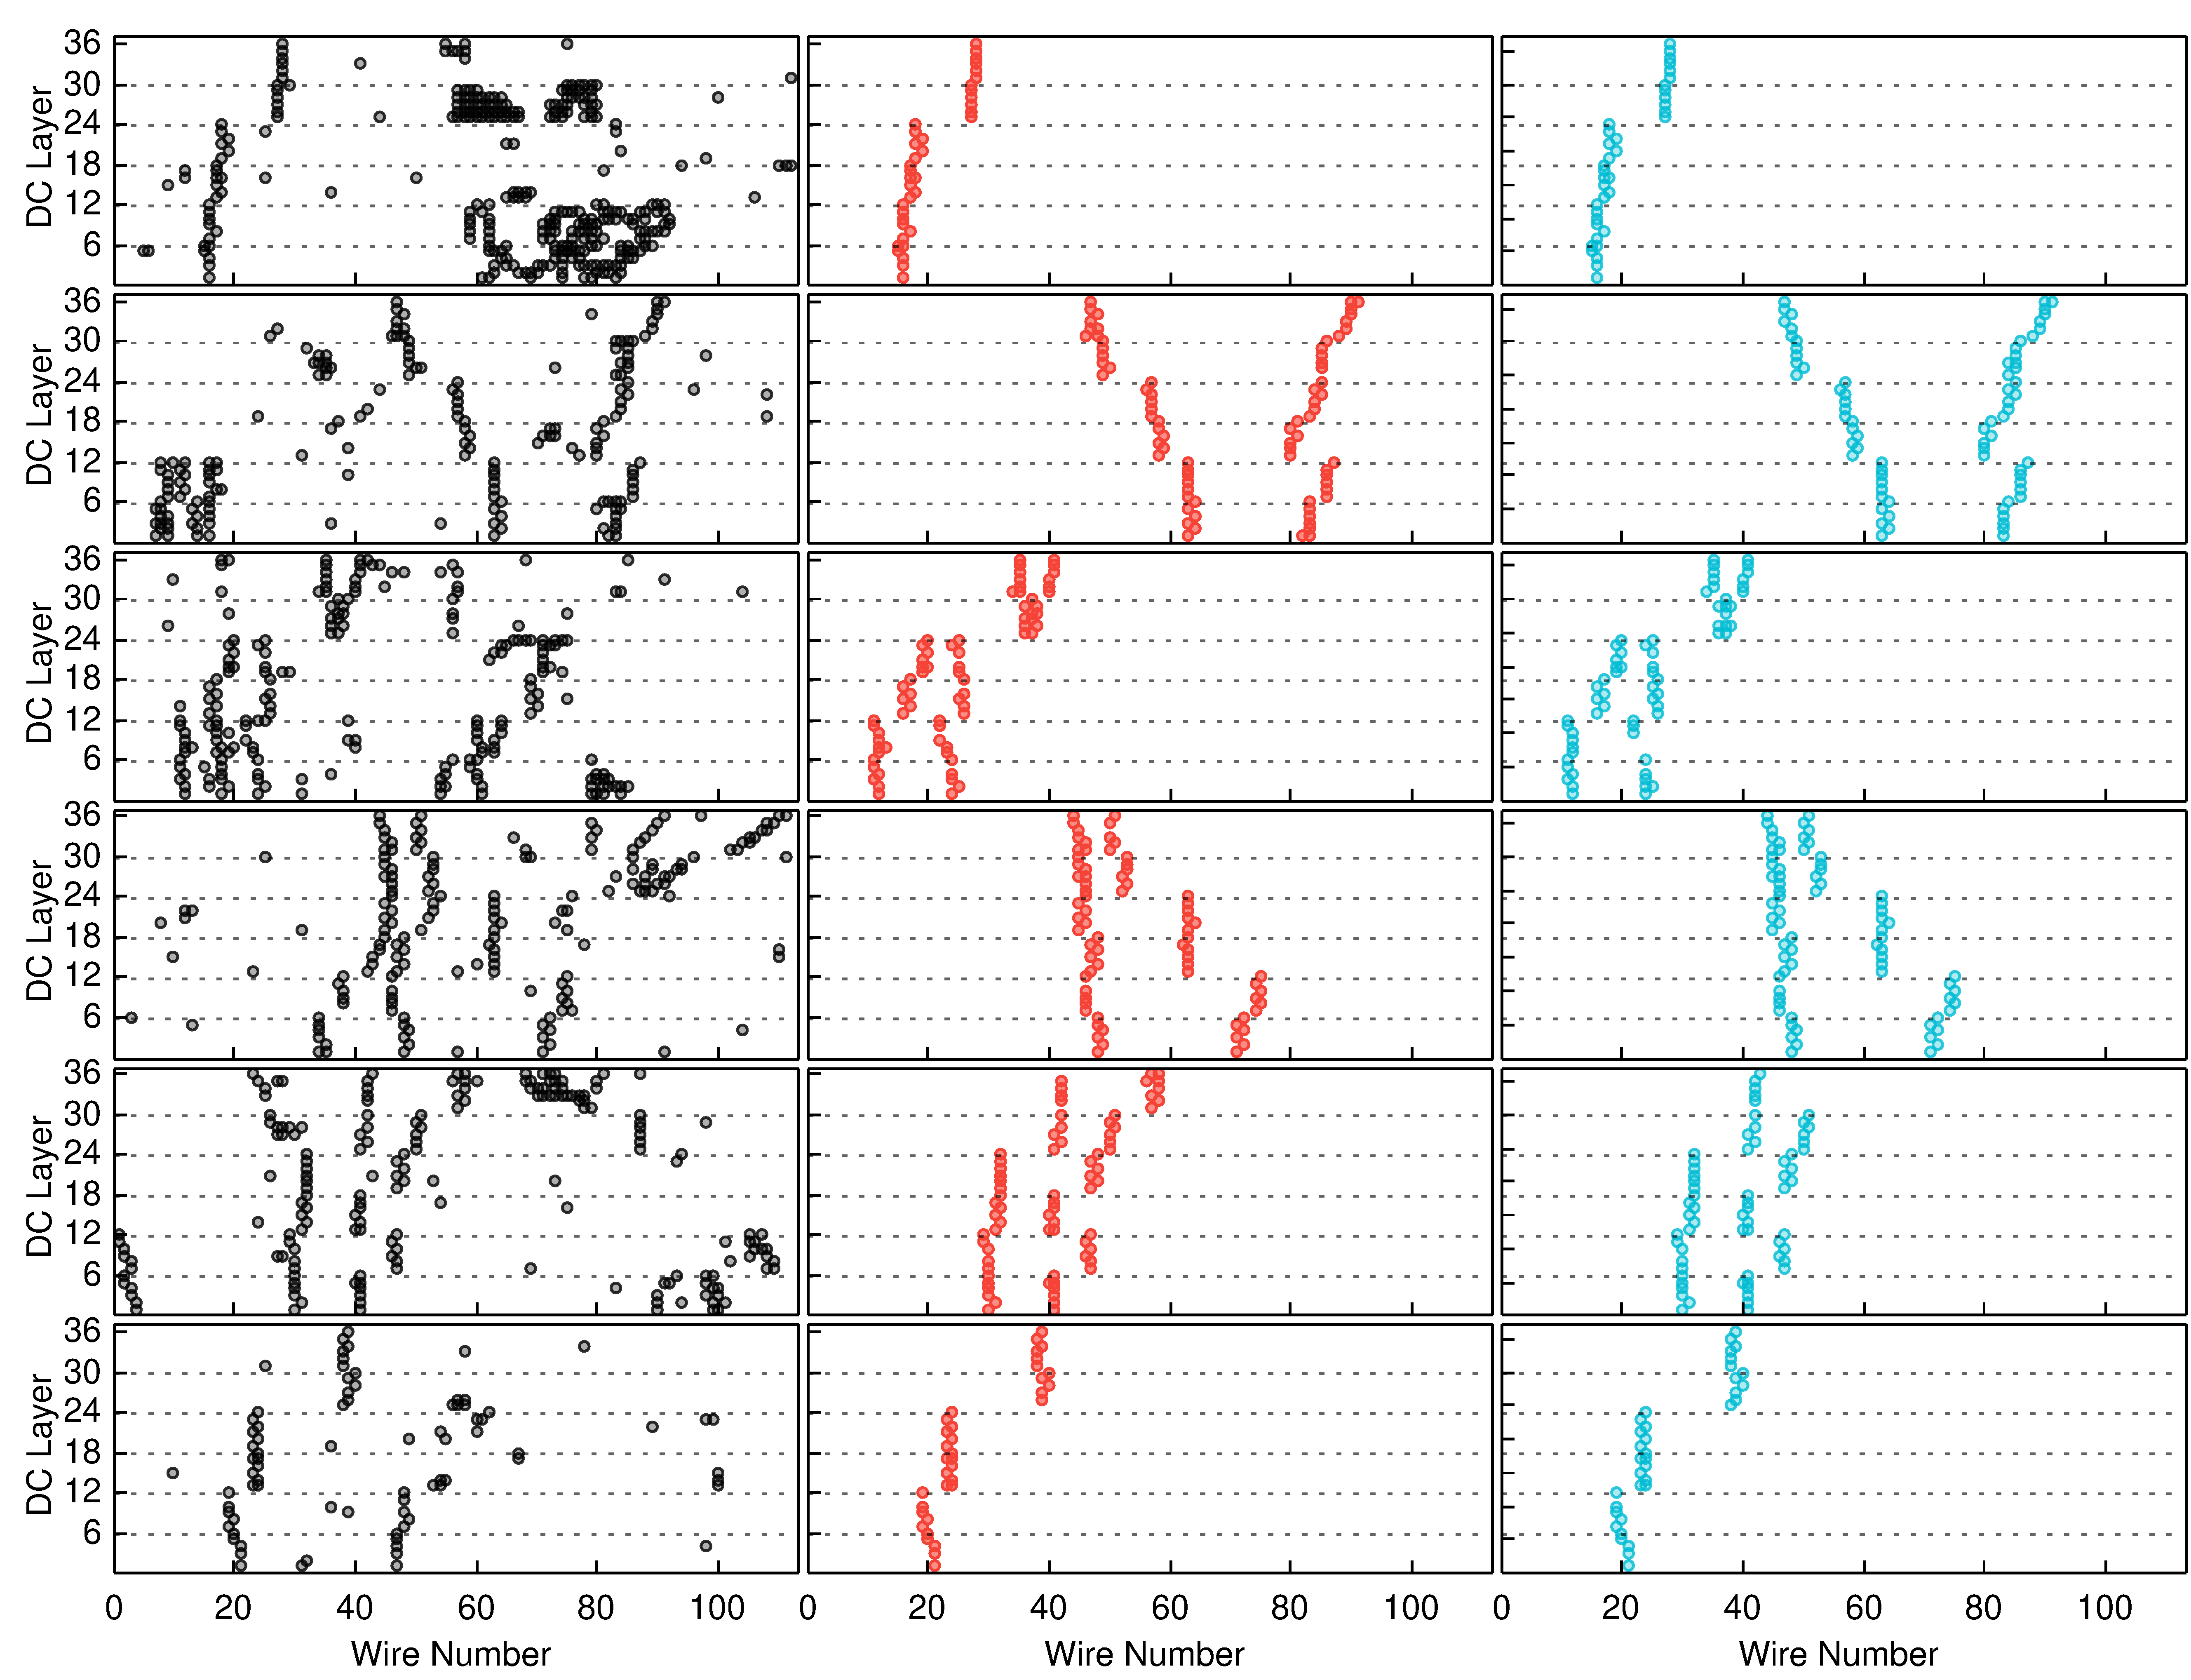
\includegraphics[width=3.8in]{images/cnn_denoise_results.pdf}
\caption {Results from the de-noising auto-encoder. The raw hits are shown
in the left column for five random events, along with hits reconstructed by the 
CLAS12 tracking algorithm in the middle column. The resulting  hits matrix 
from the de-noising raw hits are shown in the right column. (Systematic studies 
of de-noiser performance can be found here~\cite{Thomadakis:2022zcd})}
 \label{network:cnn_results}
 \end{center}
\end{figure}


\subsection{Convolutional Auto-Encoder Method}
\label{aue-method}

The Convolutional Auto-Encoder is used to de-noise raw data from the CLAS12 drift chambers~\cite{Thomadakis:2022zcd}. 
The input and output for the network are matrices of size 36x112 representing hits in one sector of drift chambers. 
The training data was extracted from experimental data processed with CLAS12 reconstruction software. 
The raw hits (converted into a matrix) are used as an input for the neural network and a matrix constructed 
only from hits that belong to reconstructed tracks as an output. 
%In the training data set multiple track hits were allowed in the output matrix, shown in Figure~\ref{conv:trackfinding}.
%The structure of the neural network can be seen in Figure~\ref{network:cnn_encoder}, where the input and the output are images
%of size 36x112. Convolutional and Max Pool layers are used for encoding the image into smaller latent space and then
%decoding it into an output image (of the same size as the input) that contains only the desired pixels activated.

%\begin{figure}[!h]
%\begin{center}
% 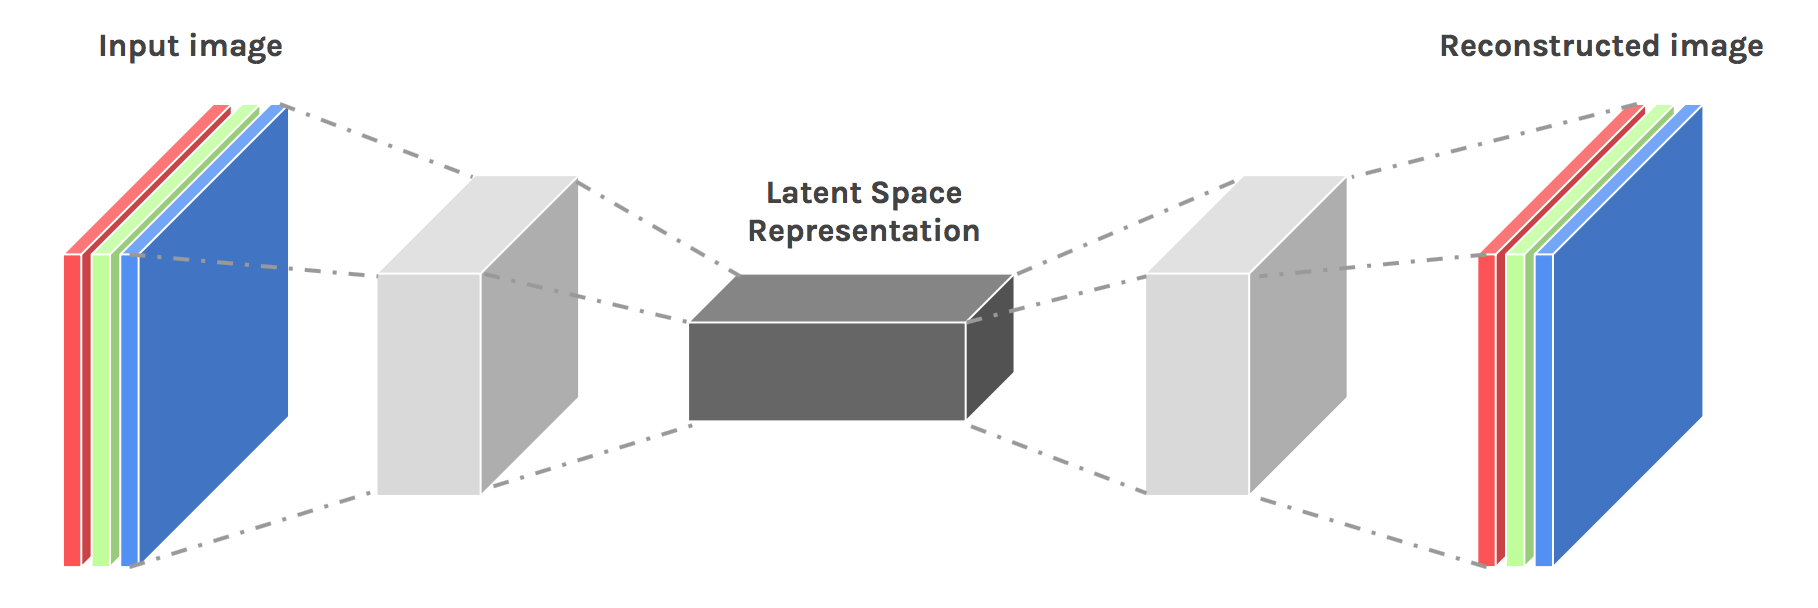
\includegraphics[width=3.1in]{images/convolutional-autoencoder.png}
%\caption {De-noising Convolutional Auto-Encoder architecture. }
% \label{network:cnn_encoder}
% \end{center}
%\end{figure}

%The networks are validated on experimental data where the number of hits along the 
%track trajectory from de-noised are compared to the hits reconstructed by the conventional algorithm
%as part of a valid track. 
An example of comparison can be seen in Figure~\ref{network:cnn_results} 
where raw data (left column) are shown along with data with hits belonging to reconstructed tracks 
identified by the conventional tracking algorithm (middle column) and 
reduced data processed by a de-noising neural network (right column).



%As can be seen from the figure, the de-noising neural network removes all background hits not 
%associated with a track, while preserving hits belonging to a track. 
Systematic studies~\cite{Thomadakis:2022zcd} showed that more than 
$95\%$ of the track-related hits are preserved in the output of de-noiser while 
background hits are significantly suppressed for normal experimental conditions of $45~nA$
incident beam current. 
%Systematic studies showed that in more than $85\%$ of cases all 
%6 clusters belonging to the track are fully identified by the algorithm after de-noising, 
%and in more than $97\%$ of the cases, 5 clusters from the original track are recovered. The CLAS12 
%track reconstruction algorithm can reconstruct tracks with 6 or 5 clusters along the 
%track trajectory, which means that even if some clusters are lost due to de-noising 
%procedure the track efficiency does not suffer significantly from this.

\subsection{Physics Impact}
\label{denoising-physics-impact}

The full chain of AI tools is implemented in the CLAS12 workflow. The reconstruction of tracks in drift chambers
starts with a De-Noising auto-encoder which removed the hits that are determined to be noise from raw DC data,
then the clustering algorithm finds clusters in the drift chambers individually for each super-layer. The clusters are 
further processed with AI-assisted tracking to find combinations of clusters that form a track. After the track candidates 
were identified the DC conventional algorithm is used to reconstruct track parameters using Kalman-Filter.

In Figure~\ref{physics::conv_dn_ai} the results from simulations are shown where the complete chain of AI was used 
to reconstruct simulated data. The simulations were done using Pythia for the final state ($e^-,\pi^+\pi^-$), and a background 
was added for different experimental conditions (luminosity). The results of the number of protons in the missing mass are shown
as a function of the beam current. As can be seen from the figure the efficiency of the proton reconstruction is significantly improved
when AI is used in track reconstruction. The results suggest that the experiments can run efficiently at higher beam currents with
AI without loss of track reconstruction efficiency.

\begin{figure}[!h]
\begin{center}
 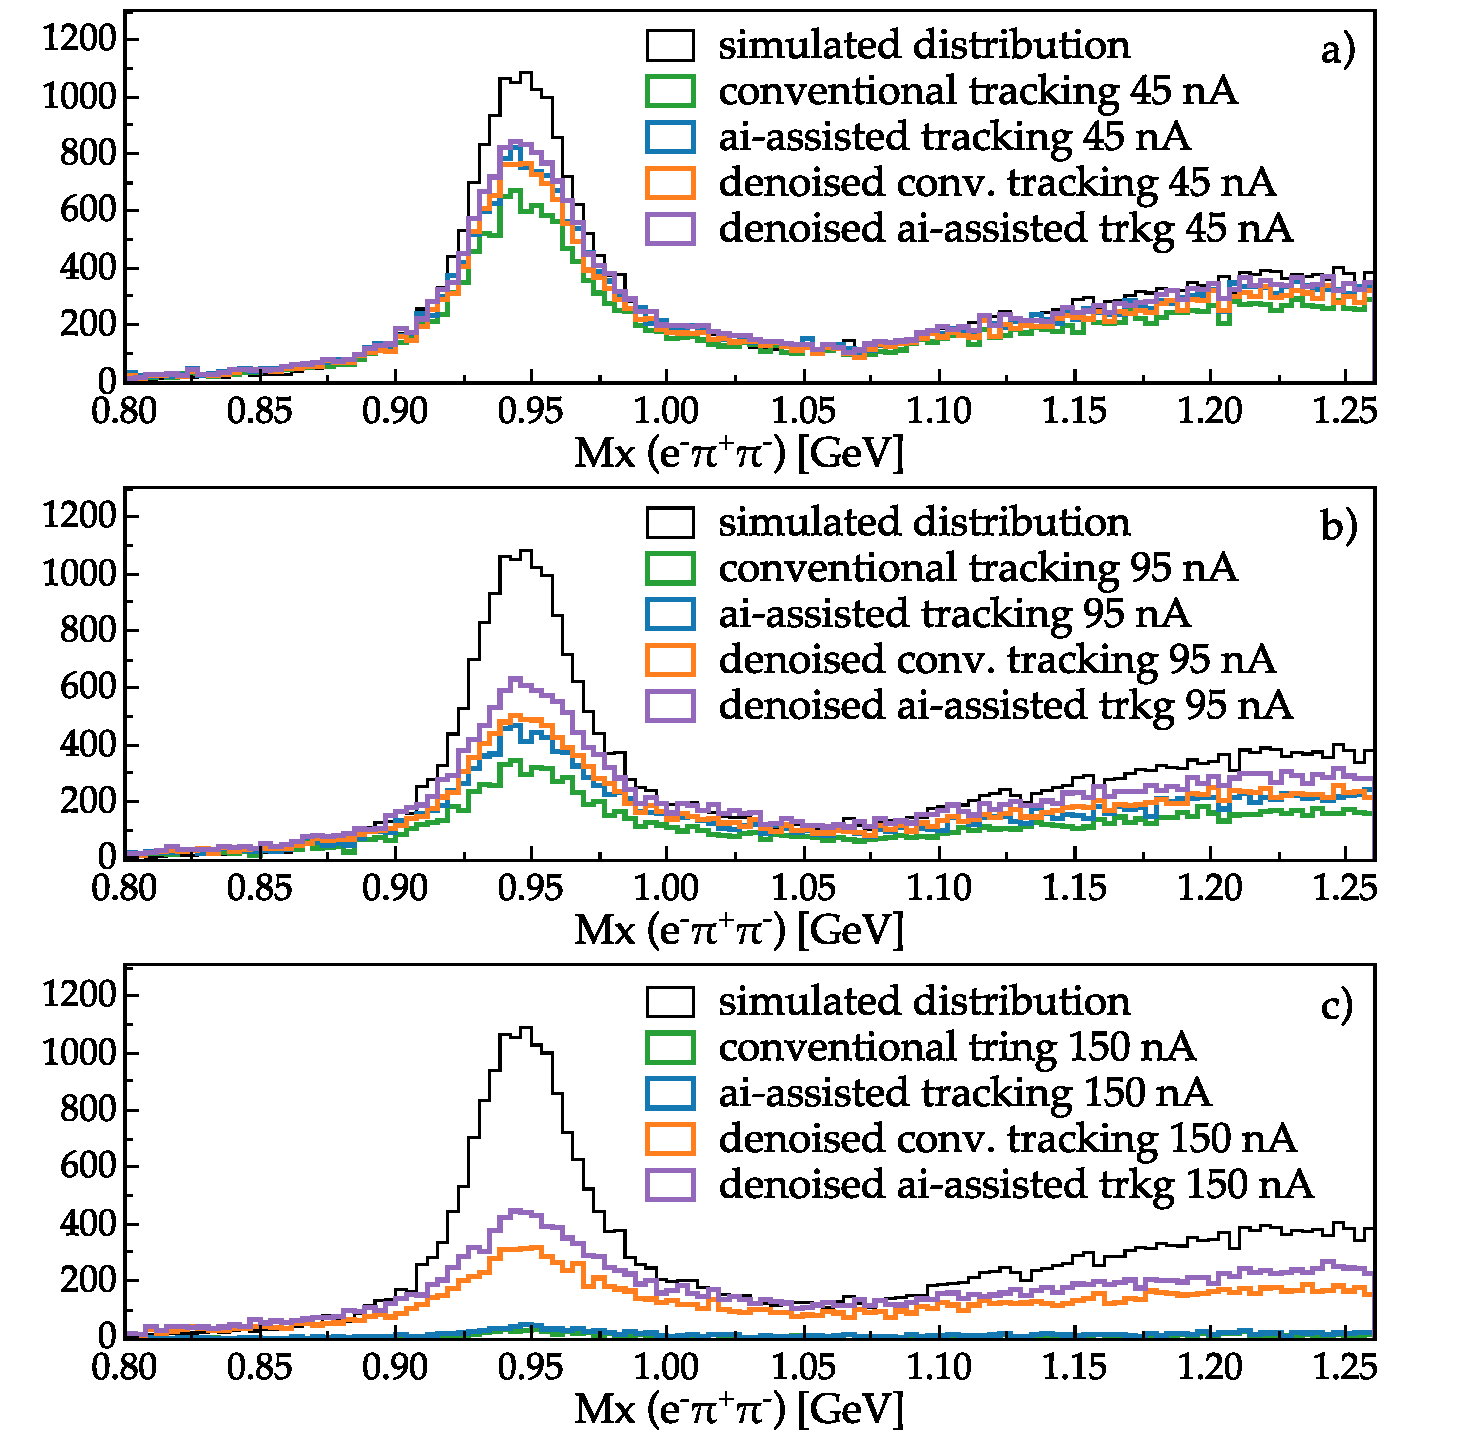
\includegraphics[height=2.in]{images/missing_mass.pdf}
 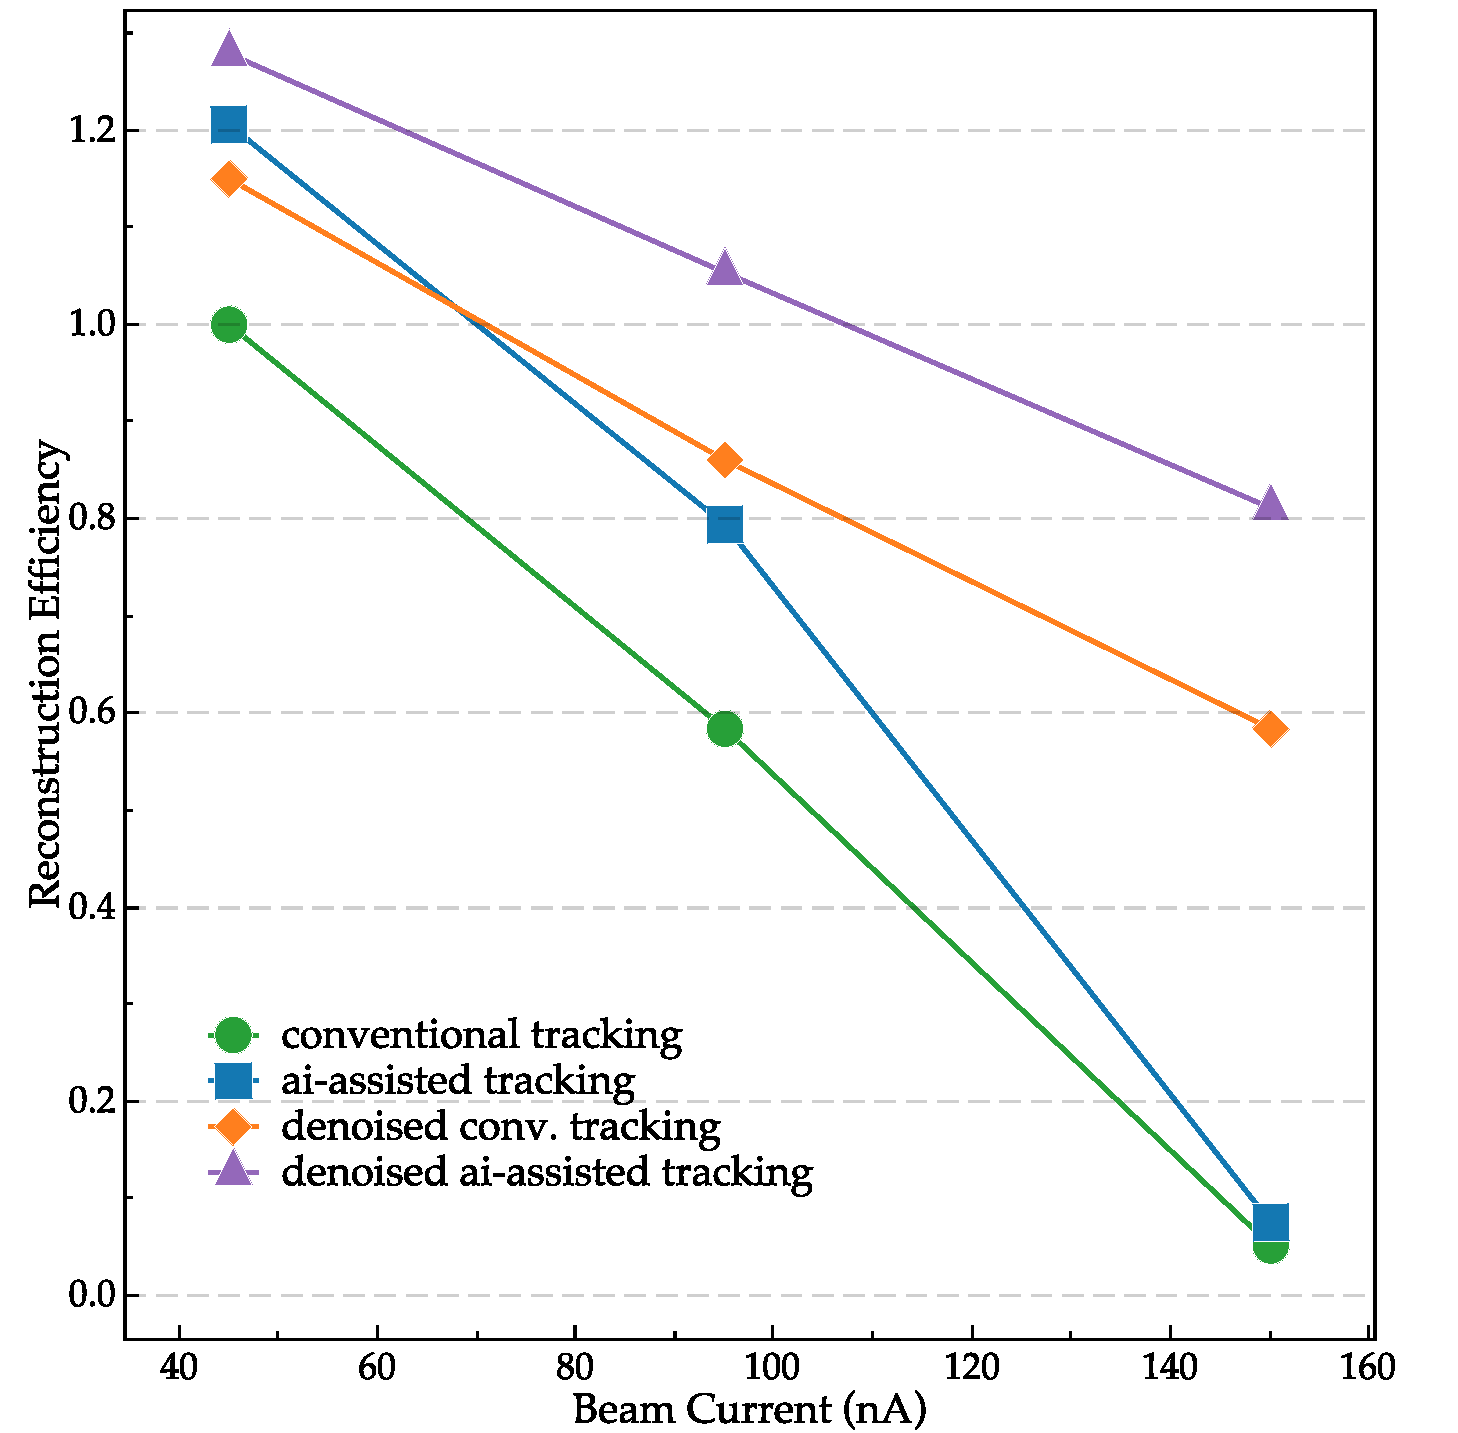
\includegraphics[height=2.in]{images/luminosity_scan.pdf}
\caption { 
The de-noised data sample was reconstructed with an AI-assisted tracking 
algorithm (triangles)  for $45~nA$, $95~nA$, and $150~nA$. a), b) and c) reconstructed missing mass distributions for 
background merged data set reconstructed with conventional tracking (filled histogram) and de-noised data sample 
reconstructed with AI-assisted algorithm (solid line histogram). Missing mass distribution for data sample before 
background merging ($0~nA$) is shown (circles) for reference.
The number of reconstructed protons from missing mass of $H(e \rightarrow e^\prime \pi^+ \pi^-) X$ 
for background merged data set reconstructed with conventional tracking (circles) compared to de-noised data sample 
reconstructed with conventional algorithm (diamonds) d). }
 \label{physics::conv_dn_ai}
 \end{center}
\end{figure}

The AI-driven track reconstruction was tested on existing experimental data (shown in Figure~\ref{physics::conv_vs_dnai}. The same final state 
was studied in experimental data (collected at standard experimental conditions of $45~nA$ beam incident on hydrogen target), and the results
show $48\%$ increase in statistics.

\begin{figure}[!h]
\begin{center}
 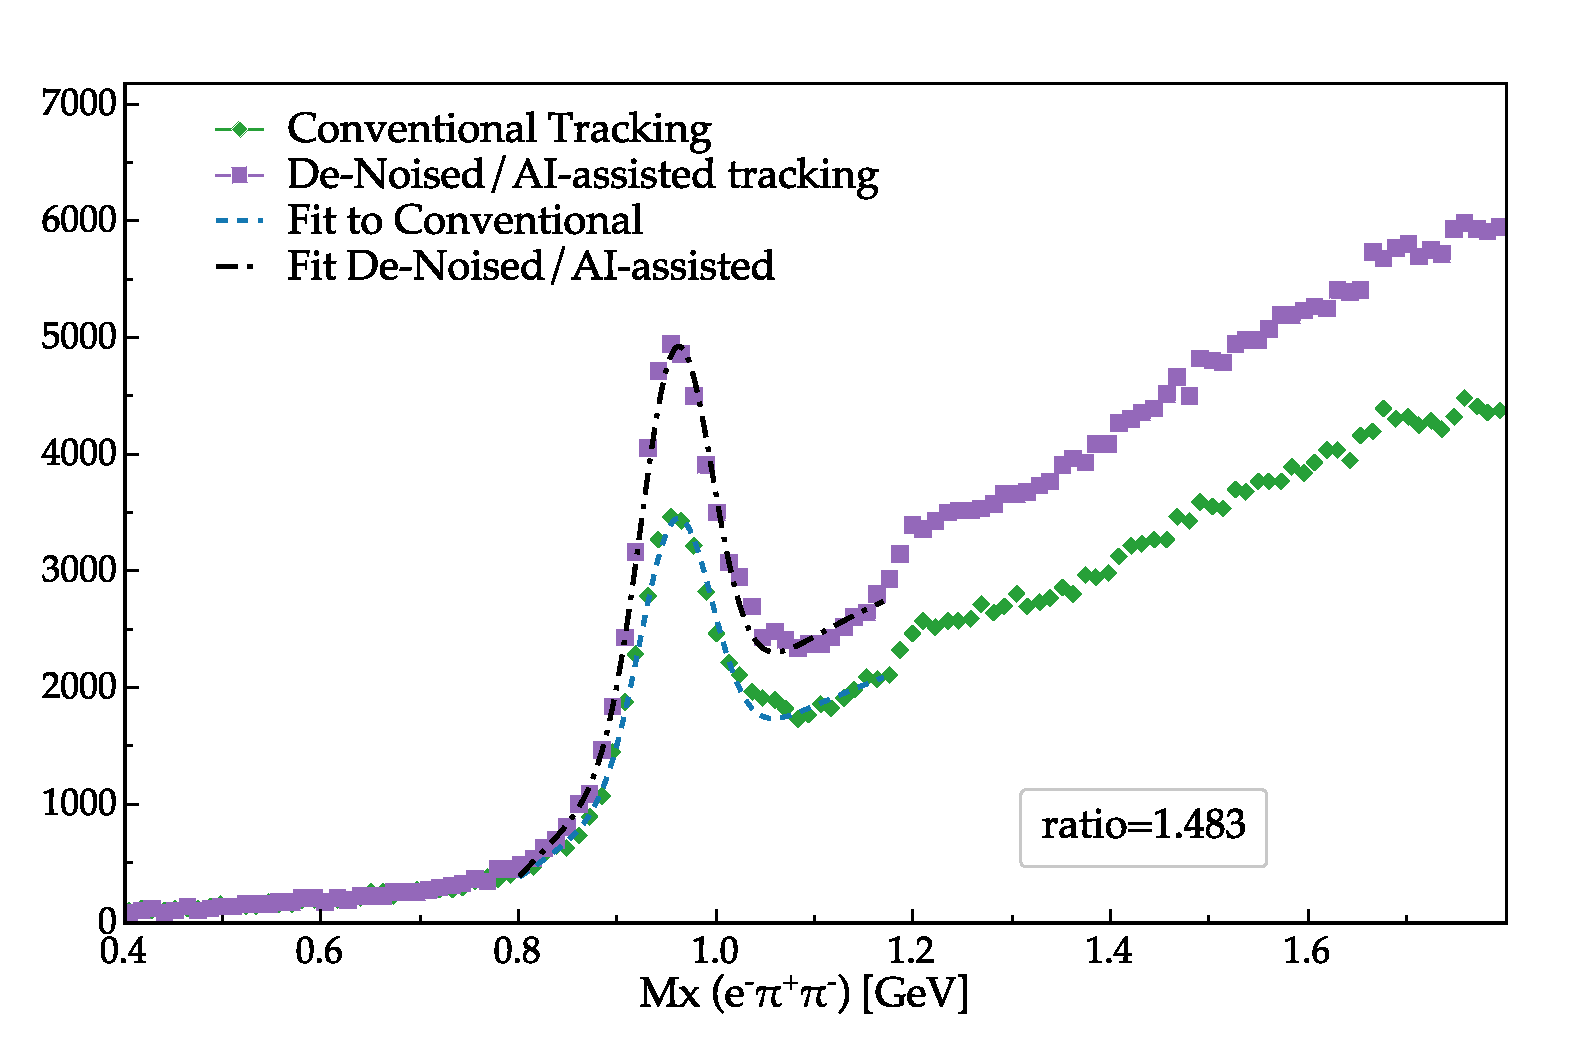
\includegraphics[height=2.in]{images/rga_conv_vs_dnai.pdf}
\caption { 
The number of reconstructed protons from missing mass of $H(e \rightarrow e^\prime \pi^+ \pi^-) X$ from experimental data 
, 45 nA beam incident on hydrogen target, is plotted to compare the number of reconstructed proton final stated from conventional tracking algorithm with 
number of protons from de-noised AI-assisted tracking. 
}
 \label{physics::conv_vs_dnai}
 \end{center}
\end{figure}

\section{Summary}
\label{section-summary}

The track reconstruction in CLAS12 currently uses AI to increase track reconstruction efficiency. The combination of De-Noising 
and AI track identification leads to a $48\%$ increase in statistics in three particle final states in experimental data. The studies 
with simulation show that upcoming experiments can be planned at higher luminosity to increase physics outcomes. 

\section{Acknowledgments}
\label{Acknowledgments}

This material is based upon work supported by the U.S. Department of Energy, Office of Science, Office of Nuclear Physics under contract DE-AC05-06OR23177, and
 NSF grant no. CCF-1439079 and the Richard T. Cheng Endowment. This work was performed using the Turing and Wahab computing clusters at Old Dominion University.
 
\begin{thebibliography}{}
%
% and use \bibitem to create references.
%
\bibitem{Burkert:2020akg}
Burkert, V.D. and others, The CLAS12 Spectrometer at Jefferson Laboratory, Nucl. Instrum. Meth. A \textbf{959},163419 (2020)
% Format for Journal Reference
%Journal Author, Journal \textbf{Volume}, page numbers (year)
% Format for books
\bibitem{Mestayer:2020saf}
 "Mestayer, M.D. and others", The CLAS12 drift chamber system, Nucl. Instrum. Meth. A",\textbf{959} 163518 (2020)
\bibitem{Kalman1960}
  Kalman, R. E., A New Approach to Linear Filtering and Prediction Problems, Journal of Basic Engineering, \textbf{82}, 35-45 (1960)
\bibitem{Gavalian:2020oxg}
Gavalian, Gagik and Thomadakis, Polykarpos and Angelopoulos, Angelos and Ziegler, Veronique and Chrisochoides, Nikos, Using Artificial Intelligence for Particle Track Identification in CLAS12 Detector, \textbf{2008.12860}, (2020)
\bibitem{Gavalian:2020xmc}
 Gavalian Gagik,Auto-encoders for Track Reconstruction in Drift Chambers for CLAS12, \textbf{2009.05144}, (2020)
\bibitem{Thomadakis:2022zcd}
   Thomadakis, Polykarpos and Angelopoulos, Angelos and Gavalian, Gagik and Chrisochoides, Nikos, De-noising drift chambers in CLAS12 using convolutional autoencoders, \textbf{271}, 108201 (2022)
%\bibitem{RefB}
%Book Author, \textit{Book title} (Publisher, place, year) page numbers
% etc
\end{thebibliography}

\end{document}

% end of file template.tex<div id='footer'><table width='100%'><tr><td class='right'><a href='http://fusioninventory.org/'><span class='copyright'>FusionInventory 9.1+1.0 | copyleft <img src='/glpi/plugins/fusioninventory/pics/copyleft.png'/>  2010-2016 by FusionInventory Team</span></a></td></tr></table></div>